\documentclass[12pt,a4paper]{ctexart}
\usepackage[a4paper,top=25mm,bottom=25mm,left=25mm,right=25mm,headheight=15pt]{geometry}
\usepackage{amsmath,amssymb,bm,booktabs,longtable,array,tabularx,multirow}
\usepackage{graphicx,float,subcaption,xcolor,hyperref,fancyhdr,enumitem,tikz}
\usepackage{tikz}
\usetikzlibrary{shapes.geometric, arrows.meta, positioning, shadows}
\usepackage{listings}
\lstset{
  language=Python,
  basicstyle=\footnotesize\ttfamily,
  keywordstyle=\color{blue!80!black}\bfseries,
  commentstyle=\color{gray!80!black}\itshape,
  stringstyle=\color{teal!80!black},
  numbers=left,
  numberstyle=\tiny\color{gray},
  stepnumber=1,
  numbersep=6pt,
  frame=single,
  framerule=0.5pt,
  rulecolor=\color{gray!30},
  backgroundcolor=\color{gray!5},
  breaklines=true,
  breakatwhitespace=true,
  tabsize=4,
  columns=flexible,
  xleftmargin=1.5em,
  xrightmargin=0.5em
}
\usepackage{setspace}
\newcommand{\problem}[1]{\par\noindent\hspace*{2em}\textbf{针对问题#1}\quad}
\graphicspath{{figures/}}
\hypersetup{colorlinks=true,linkcolor=black,citecolor=black,urlcolor=blue}
\setstretch{1.30}
\setlength{\parindent}{2em}
\setlength{\parskip}{0pt}
\setlist{nosep,leftmargin=2em}
\pagestyle{fancy}
\fancyhf{}
\cfoot{\thepage}
\renewcommand{\headrulewidth}{0pt}
\newcommand{\QThreeDryHours}{57.5303}
\newcommand{\QFourDryHours}{52.6776}
\newcommand{\AppendixFourFixedHours}{129.9873}
\newcommand{\NoCoordinateCaseHours}{51.1141}
\newcommand{\ShrinkReduction}{59.47\%}
\newcommand{\AppendixIncrease}{125.95\%}
\newcommand{\OmitCoordinateDifference}{-2.97\%}
\newcommand{\NetReduction}{8.44\%}
\newcommand{\StableStartHours}{2.050}
\newcommand{\PlateauTemperature}{50.0049}
\newcommand{\PlateauMoisture}{0.049994}
\newcommand{\QFourDryRadius}{1.2000}
\newcommand{\ConservationError}{1.61e-15}
\newcommand{\EquilibriumError}{2.06e-11}
\newcommand{\QThreeGridChange}{0.092\%}
\newcommand{\QFourGridChange}{0.045\%}
\newcommand{\QFourTimeChange}{0.00148\%}
\newcommand{\QOneMoistureProfileError}{8.69e-05}
\newcommand{\QTwoMoistureProfileError}{2.92e-06}


\title{\vspace{-2.2em}\bfseries 基于热质耦合的药材烘干模型}
\author{}
\date{}

\begin{document}
\maketitle
\vspace{-4em}

\begin{abstract}
药材烘干过程同时涉及内部的热传导、水分扩散和表面的对流换热、传质，并伴随材料物理性质及几何尺寸的变化。如何准确描述药材内部温度与水分浓度的演化，进而确定满足要求的烘干时长，是优化烘干工艺、降低能耗并保证产品品质的关键。本文将药材视为细长圆柱体，忽略远离端面位置的轴向梯度，建立一维径向热质传递模型；然后采用有限体积法完成空间离散，将偏微分方程组降维成常微分方程组，并利用后向差分公式（Backward Differentiation Formula, BDF）进行自适应时间积分。在此基础上，依次研究恒定物理性质、非线性热质耦合、烘干终止判定以及半径动态收缩条件下的数值求解问题。

\problem{一}首先根据圆柱药材长度较长的几何特征，将温度和水分浓度近似为仅随径向位置和时间变化的函数。对于预热阶段，建立线性热传导方程与扩散系数随含水率变化的非线性水分扩散方程，在圆心处设置对称边界，并在表面设置对流换热、传质的 Robin 边界条件。利用附件中的烘房温度和水分浓度数据构造分段线性插值函数，用有限体积法把半径离散，再通过 BDF 求解离散后的常微分方程组，得到 $0\sim1800\,\mathrm{s}$ 内药材各径向位置的温度与水分浓度变化规律。计算表明，预热过程中药材表面温度上升快于中心温度，水分浓度呈现中心高、表面低的径向分布。在 $t=1800\,\mathrm{s}$ 时，对应 $r=(0,\,0.5,\,1.0,\,1.5,\,2.0)\,\mathrm{cm}$ 处的计算结果为：温度向量 $\bm T_{1800}=(33.5754,\allowbreak\, 33.7721,\allowbreak\, 34.3641,\allowbreak\, 35.3622,\allowbreak\, 36.7859)\,{}^\circ\mathrm C$；含水率向量 $\bm C_{1800}=(2.5500,\allowbreak\, 2.5497,\allowbreak\, 2.5383,\allowbreak\, 2.3755,\allowbreak\, 1.5103)\,\mathrm{kg/kg}$。

\problem{二}在问题一的基础上，建立参数随温度、含水率变化的非线性热质耦合模型。对相邻节点间的导热系数和扩散系数采用调和平均，从而保证跨界面通量连续；将烘房环境划分为动态预热段与稳定恒温段，前段用附件数据插值，后段近似取 $T_a^*=50\,{}^\circ\mathrm C$、$C_a^*=0.05\,\mathrm{kg/kg}$。采用 $\Delta r=0.05\,\mathrm{cm}$ 的细网格求解，并进行时空插值和结果输出，最终得到前 $3\,\mathrm h$ 内药材温度与水分浓度的演化曲线。当 $t=3\,\mathrm h$ 时，中心与表面的计算结果为：$T_{\mathrm c}=49.8484\,{}^\circ\mathrm C$，$T_{\mathrm s}=49.8975\,{}^\circ\mathrm C$；$C_{\mathrm c}=1.7658\,\mathrm{kg/kg}$，$C_{\mathrm s}=1.0080\,\mathrm{kg/kg}$。

\newpage
\problem{三}在问题二基础之上，将烘干完成条件定义为全场最大含水率低于目标阈值，即 $t_{\mathrm{dry}}=\inf\{\,t>0:\ \max_{0\le r\le R_0}C(r,t)<0.15\,\mathrm{kg/kg}\,\}$。在 BDF 求解器中设置终止事件，并将仿真时间延长至所有径向节点均满足阈值。数值结果显示，药材中心的水分浓度始终最大，是决定烘干时长的控制位置。连续阈值时刻为 $207246.43\,\mathrm{s}$（$57.5685\,\mathrm h$）；取首个严格达标的 $60\,\mathrm{s}$ 输出时刻，最终烘干时间为 $207300\,\mathrm{s}$（$57.5833\,\mathrm h$）。此时各指定位置的水分浓度为 $\bm C_{\mathrm{dry}}=(0.1500,\allowbreak\,0.1477,\allowbreak\,0.1402,\allowbreak\,0.1250,\allowbreak\,0.0525)\,\mathrm{kg/kg}$，依次对应 $r=(0,\,0.5,\,1.0,\,1.5,\,2.0)\,\mathrm{cm}$。未舍入的最大值为 $0.14998444\,\mathrm{kg/kg}$，满足严格阈值条件。

\problem{四}该问题需同时考虑药材失水引起的径向收缩。依据附件半径数据构造 $R(t)$ 的分段线性插值函数，并引入无量纲坐标 $\xi=r/R(t)$（$0\le \xi\le 1$），将随时间变化的物理区域映射至固定计算区间。坐标变换后，在热传导与水分扩散方程中加入网格运动项 $\xi\dot R(t)/R(t)$ 及尺度因子 $1/R^2(t)$，结合附录四给出的物性关系，在固定 $\xi$ 网格上继续采用有限体积法与 BDF 求解，并以 $\max_i C_i<0.15\,\mathrm{kg/kg}$ 作为终止条件。为区分物性变化与几何收缩的影响，分别计算“固定半径--附录三物性”“固定半径--附录四物性”和“动态半径--附录四物性”三组方案。完整收缩模型的主要结果为：连续理论达标时刻 $t_{\mathrm{continuous}}=189768.43\,\mathrm{s}$（$52.7135\,\mathrm h$），安全输出时刻 $t_{\mathrm{dry}}=189780\,\mathrm{s}$（$52.7167\,\mathrm h$），此时药材半径收缩至 $R(t_{\mathrm{dry}})=1.2000\,\mathrm{cm}$，最大含水率 $\max_i C_i=0.14999407\,\mathrm{kg/kg}$。与问题三相比，烘干时长缩短 $17520\,\mathrm{s}$（$4.8667\,\mathrm h$），降幅为 $8.45\%$；与采用附录四物性但保持固定半径的对照模型相比，烘干时长缩短 $77.3000\,\mathrm h$，降幅为 $59.45\%$，干燥速度提高至原来的 $2.466$ 倍。结果说明，径向收缩通过缩短水分扩散距离显著提高了烘干效率。

最后给出了建模过程的误差分析和结果检验，本文结论正确合理，具有一定的应用价值和普适性。

\vspace{0.6em}
\noindent\textbf{关键词：}热质耦合；有限体积法；BDF；非线性扩散；移动边界；药材烘干
\end{abstract}
\clearpage

\section{问题重述}

\subsection{问题背景}

干燥是中药材加工过程中影响成品品质的重要工序。该工艺通常经历预热平衡和恒温干燥两个阶段：烘房通过调节温度与水分浓度，使热量由药材表面逐渐向内部传递，同时促使内部水分向外扩散并由热风带走。药材内部温度场和水分浓度场的变化相互关联，其演化过程还会受到材料物性、外部环境以及药材尺寸变化等因素的共同影响。

在实际生产中，若烘干参数设置不合理，容易出现干燥时间过长、能源利用率偏低以及内外干燥程度不一致等问题，进而影响药材质量。传统的试验优化方法需要反复调整工艺，不仅成本较高，而且周期较长。因此，有必要根据传热传质机理建立数学模型，借助数值计算刻画药材内部温度和水分浓度的变化规律，并进一步预测烘干完成时间，为烘干工艺的分析与优化提供依据。

\subsection{题目重述}

现有某种中药材，其外形可近似看作长为 $25\,\mathrm{cm}$、半径为 $2\,\mathrm{cm}$ 的圆柱体。烘干开始时，药材内部温度均为 $28\,{}^\circ\mathrm{C}$，水分浓度（干基含水率）均为 $2.55\,\mathrm{kg/kg}$。烘房在烘干初期的温度和水分浓度随时间变化，药材的密度、比热容、热传导系数及水分扩散系数在不同阶段采用不同的经验关系；与此同时，药材还会因水分流失而产生径向收缩。现需根据题目给出的环境数据、半径数据及相关物性参数，研究以下四个问题。

\textbf{问题一：}针对预热平衡阶段，分析外部烘房环境变化对圆柱药材内部传热、传质过程的影响，建立药材温度和水分浓度随时间及径向位置变化的数学模型。计算 $0\sim1800\,\mathrm{s}$ 内药材内部的温度场和水分浓度场，给出题目指定时刻及距中心 $0$、$0.5$、$1$、$1.5$、$2\,\mathrm{cm}$ 处的结果，并按规定的时间、空间间隔保存完整数据。

\textbf{问题二：}考虑烘干过程一般持续 $2\sim3$ 天，且预热平衡阶段与恒温干燥阶段的环境和物性特征存在差异。采用题目给出的统一经验公式，建立能够描述整个烘干过程的温度--水分耦合模型，求出前 $3\,\mathrm{h}$ 内药材各处温度和水分浓度的变化情况，并输出指定时刻、指定径向位置及完整时空网格上的计算结果。

\textbf{问题三：}在问题二所建立的全过程模型基础上，以药材内部所有位置的水分浓度均低于 $0.15\,\mathrm{kg/kg}$ 作为烘干完成标准，确定满足该条件所需要的烘干时长。给出烘干过程中每隔 $6\,\mathrm{h}$、距中心每隔 $0.5\,\mathrm{cm}$ 的水分浓度，并按题目要求保存全过程的水分浓度数据。

\textbf{问题四：}进一步考虑药材在失水过程中发生的尺寸收缩，根据附件所给半径随时间的变化数据以及新的物性经验公式，对问题三的模型进行修正。在变化区域内重新计算药材水分浓度的时空分布，确定考虑尺寸变化后的烘干时长，并给出指定时刻、指定位置及药材表面处的水分浓度，同时形成规定格式的完整结果文件。



\section{问题分析}

药材烘干本质上是热量传递与水分迁移同步进行的非稳态过程，二者具有明显的\textbf{热质相似性}。热传导遵循傅里叶定律，水分扩散遵循菲克定律；对于轴对称圆柱药材，其控制方程均可写成“局部积累量等于径向净通量”的形式：
\begin{equation}
 \rho c_p\frac{\partial T}{\partial t}
 =\frac{1}{r}\frac{\partial}{\partial r}
 \left(rk\frac{\partial T}{\partial r}\right),\qquad
 \frac{\partial C}{\partial t}
 =\frac{1}{r}\frac{\partial}{\partial r}
 \left(rD\frac{\partial C}{\partial r}\right).
\end{equation}
其中，温度 $T$ 与水分浓度 $C$、热传导系数 $k$ 与水分扩散系数 $D$、表面对流换热系数 $h$ 与传质系数 $h_m$ 分别构成对应关系。两类场在圆柱中心均满足对称条件，在药材表面均满足第三类边界条件。因此，可在统一的径向控制体积网格上离散温度场与水分场，再通过材料物性随 $C$、$T$ 的变化体现二者之间的耦合。需要注意的是，热量由高温处向低温处传递，而水分由高浓度处向低浓度处扩散，二者的量纲、扩散速率及外部驱动力并不相同，故只能共享建模框架，不能将两种传递过程简单等同。

基于上述相似性，本文将药材视为长径比较大的圆柱体，忽略轴向与周向差异，重点研究温度和水分浓度沿半径方向的变化。空间上采用有限体积法离散，使每个控制体均保持能量与质量守恒；时间上将偏微分方程组转化为常微分方程组，并采用适用于刚性系统的 BDF 方法求解。四个问题由“固定半径下的短时预热”逐步推广至“物性变化的全过程烘干”和“考虑收缩的移动边界烘干”，前一问所得模型为后一问提供基础。

\subsection{问题一分析}

问题一要求在给定烘房温度和水分浓度变化条件下，计算预热平衡阶段药材内部温度场与水分浓度场，并给出指定时刻和径向位置上的结果。该问题的关键在于：外界环境随时间变化，水分扩散系数又随局部含水率改变，因而即使材料的热学参数取常数，整个传热传质过程仍具有时变边界和非线性扩散的特征。

首先，根据药材几何尺寸及长圆柱假设，分别建立一维径向热传导方程和水分扩散方程；将附件给出的烘房温度、烘房水分浓度数据作分段线性插值，作为药材表面的动态边界条件。圆柱中心处由于 $r=0$，控制方程含有形式上的奇点，应利用中心控制体的守恒关系进行单独离散；药材表面则分别建立对流换热与对流传质条件。

其次，在同一径向网格上利用有限体积法计算各控制体之间的热通量与水分通量，得到药材各离散位置温度和水分浓度随时间变化的方程组。由于扩散系数 $D(C)$ 随求解结果实时变化，采用隐式 BDF 方法进行时间积分，以提高非线性刚性系统长时间计算的稳定性。最后，利用数值解的连续输出功能读取题目指定时刻和位置的结果，并按规定的时间、空间间隔形成完整数据文件。为排除网格尺寸对结果的显著影响，还需比较网格加密前后的最大误差，验证离散结果已经基本稳定。

\subsection{问题二分析}

问题二将计算范围由 $1800\,\mathrm{s}$ 的预热平衡阶段扩展到持续 $2\sim3$ 天的完整烘干过程。与问题一相比，药材的密度、比热容、热传导系数均随水分浓度改变，水分扩散系数同时受温度和水分浓度影响。因此，该问题不再是两个相互独立的扩散方程，而是物性参数不断更新的非线性热质耦合问题。

在问题一模型的基础上，采用附件三给出的 $\rho(C)$、$c_p(C)$、$k(C)$ 与 $D(C,T)$ 经验关系替换常参数，并在每一个时间步根据当前温度场和水分场更新材料物性。相邻控制体界面处的热传导系数和水分扩散系数采用调和平均，以保证通量连续并减小物性突变引起的数值误差。烘房环境则按实际工艺划分为预热变化阶段和随后近似稳定的恒温干燥阶段。

空间离散后，温度和水分浓度共同组成耦合常微分方程组。由于全过程时间尺度较长，而早期温度变化与后期水分缓慢迁移的时间尺度差异明显，仍采用具有自适应步长的 BDF 方法进行求解。和问题一相比，无需重新构造数值框架，只需更新材料物性与外界条件，即可得到前 $3\,\mathrm{h}$ 及完整烘干时段内的温度、水分浓度分布。

\subsection{问题三分析}

问题三要求确定药材内部所有位置的水分浓度均低于 $0.15\,\mathrm{kg/kg}$ 时的烘干时长。该问实质上不是建立新的控制方程，而是在问题二全过程耦合模型上增加终止判据，将定时长仿真转化为未知终止时刻的事件求解问题。

由于药材表面直接与干燥空气接触，通常比内部更早达到目标含水率，靠近中心的位置可能成为决定烘干完成时间的关键。但为避免仅考察中心点造成误判，应以全部离散位置中的最大水分浓度作为判定指标，即构造
\begin{equation}
 g(t)=\max_i C_i(t)-0.15.
\end{equation}
当 $g(t)$ 首次由正值降至零时，说明所有位置均已满足干燥标准，此时对应的时刻即为所求烘干时长。计算时继续沿用问题二的有限体积离散与 BDF 积分，并启用终止事件自动捕捉临界时刻；随后利用稠密输出提取每隔 $6\,\mathrm{h}$、各指定半径处的水分浓度，从而同时给出烘干时长和全过程分布结果。

\subsection{问题四分析}

问题四进一步考虑药材失水收缩，使计算区域的半径随时间变化。此时水分扩散不仅取决于局部浓度梯度，还受到边界移动以及扩散距离缩短的影响。因此，该问题是在问题三基础上的移动边界非线性扩散问题，其难点在于原有固定径向网格不能直接适用于不断变化的物理区域。

首先，根据附件二的半径数据构造分段线性函数 $R(t)$，并引入无量纲坐标
\begin{equation}
 \xi=\frac{r}{R(t)},\qquad 0\leq \xi\leq 1,
\end{equation}
把随时间收缩的物理区域映射到固定计算区间。坐标变换后，控制方程中除原有的扩散项外，还会出现由 $\dot R(t)$ 引起的网格运动项；表面传质边界中的空间尺度也应随 $R(t)$ 同步修正。随后采用附件四给出的新物性公式，在固定的 $\xi$ 网格上重新进行有限体积离散，并继续使用 BDF 方法推进时间。

最后，以变半径模型中 $\max_i C_i(t)=0.15$ 作为烘干终止条件，求得考虑尺寸变化后的烘干时长。输出时将无量纲位置换算为各时刻的实际半径，同时单独保留药材表面节点的数据，以满足题目对指定时刻、指定位置及表面含水率的要求。将本问结果与问题三对比，还可分析径向收缩对扩散距离、内部水分迁移速度和总烘干时间的影响。



\section{模型假设}
\begin{enumerate}[
  label=\arabic*.,
  leftmargin=1.22cm,
  labelsep=0.28cm,
  itemsep=0.10cm,
  topsep=0pt,
  parsep=0pt
]

  \item 假设药材为半径 $2\,\mathrm{cm}$、长度 $25\,\mathrm{cm}$ 的规则圆柱体，材料连续、均匀且各向同性，内部无裂纹、孔洞及热源或水分源。

  \item 假设药材的初始温度和初始含水率均匀，且外界热风沿圆周方向均匀分布，因此温度场和含水率场均具有轴对称性。

  \item 假设药材内部仅考虑 Fourier 热传导和 Fick 有效水分扩散，表面仅考虑与环境之间的对流换热和对流传质；忽略热辐射、内部空气对流及压力驱动渗流。

  \item 假设各阶段环境温度、相对湿度以及表面对流换热、传质系数在给定时段内保持稳定，药材表面不存在额外接触热阻。

  \item 在不考虑收缩的阶段，假设药材几何尺寸保持不变；考虑收缩时，假设截面始终保持圆形并沿径向均匀收缩，忽略翘曲、开裂及各向异性变形。

\end{enumerate}

\section{符号说明}
\begin{table}[H]
\centering
\caption{主要符号说明}\label{tab:symbols}
\small
\renewcommand{\arraystretch}{1.1}
\begin{tabularx}{0.92\textwidth}{c<{\centering}X<{\raggedright}c<{\centering}}
\toprule
符号 & 含义 & 单位\\
\midrule
$r$ & 到药材中心的距离 & m\\
$R$ & 药材半径 & m\\
$\xi$ & 相对坐标 & --\\
$T$ & 药材内部温度 & K\\
$C$ & 药材干基含水率 & kg/kg\\
$T_a$ & 烘房环境温度 & K\\
$C_a$ & 烘房环境水分浓度 & kg/kg\\
$\rho$ & 药材表观密度 & $\mathrm{kg/m^3}$\\
$c_p$ & 药材定压比热容 & $\mathrm{J/(kg\cdot K)}$\\
$k$ & 药材导热系数 & $\mathrm{W/(m\cdot K)}$\\
$D$ & 水分有效扩散系数 & $\mathrm{m^2/s}$\\
$h$ & 表面对流换热系数 & $\mathrm{W/(m^2\cdot K)}$\\
$h_m$ & 表面对流传质系数 & m/s\\
$N$ & 径向网格划分区间数 & --\\
$\Delta r$ & 物理空间网格步长 & m\\
$\Delta\xi$ & 相对坐标空间步长 & --\\
$\Delta t$ & 时间推进步长 & s\\
$\omega_i^r$ & 物理控制体几何权重 & $\mathrm{m^2}$\\
$\omega_i^\xi$ & 相对坐标控制体几何权重 & --\\
$\Gamma$ & 广义界面传递系数 & $\mathrm{W/(m\cdot K)}$ 或 $\mathrm{m^2/s}$\\
$t_d$ & 干燥达标理论临界时刻 & h\\
$t_{\mathrm{safe}}$ & 60\,s 网格安全达标时刻 & h\\
\bottomrule
\end{tabularx}
\end{table}

\section{模型建立}
药材的热风烘干过程本质是热量由烘房向药材内传导、水分由药材内向表面迁移并蒸发两个过程的耦合。热量扩散的过程称为传热，水分扩散的过程称为传质，两者具有很强的相似性。传热满足 Fourier 导热定律和能量守恒；传质的过程满足 Fick 定律和质量守恒。

\begin{figure}[H]
\centering
\begin{tikzpicture}[scale=0.95, >=stealth]
    % Cylinder fills
    \fill[blue!5] (-1.5, -2) -- (-1.5, 2) arc (180:360:1.5 and 0.45) -- (1.5, -2) arc (0:-180:1.5 and 0.45);
    \fill[blue!15] (0, 2) ellipse (1.5 and 0.45);

    % Top ellipse
    \draw[thick, fill=blue!15] (0,2) ellipse (1.5 and 0.45);
    \fill (0,2) circle (1.5pt) node[below=2pt, font=\footnotesize] {$O$};

    % Bottom arcs
    \draw[thick] (-1.5,-2) arc (180:360:1.5 and 0.45);
    \draw[dashed, gray!70] (-1.5,-2) arc (180:0:1.5 and 0.45);

    % Cylinder sides
    \draw[thick] (-1.5,2) -- (-1.5,-2);
    \draw[thick] (1.5,2) -- (1.5,-2);

    % Center axis
    \draw[dashdotted, gray!60, thick] (0, 3.0) -- (0, -3.0) node[below, font=\footnotesize] {中心对称轴 ($r=0$)};

    % Radius R0 dimension above the top ellipse
    \draw[gray!70] (0, 2) -- (0, 2.7);
    \draw[gray!70] (-1.5, 2) -- (-1.5, 2.7);
    \draw[<->, thick, red!80!black] (0, 2.6) -- (-1.5, 2.6) node[midway, above=1pt, font=\small] {$R_0=2\,\mathrm{cm}$};

    % Length dimension on the left
    \draw[gray!70] (-1.5, 2) -- (-2.2, 2);
    \draw[gray!70] (-1.5, -2) -- (-2.2, -2);
    \draw[<->, thick, teal!80!black] (-2.1, -2) -- (-2.1, 2) node[midway, left=1pt, font=\small] {$L=25\,\mathrm{cm}$};

    % Labels for side and end faces (on the right)
    % Top end face
    \draw[<-, thick, blue!80!black] (0.8, 2.1) to[out=30, in=180] (2.4, 2.6) node[right, font=\small] {端面（顶部端面，截面积 $A_{\text{end}}$）};
    % Side surface
    \draw[<-, thick, blue!80!black] (1.5, 0.0) -- (2.4, 0.0) node[right, font=\small] {侧面（圆柱周向侧表面 $A_{\text{side}}$）};
    % Bottom end face
    \draw[<-, thick, blue!80!black] (0.8, -2.1) to[out=-30, in=180] (2.4, -2.6) node[right, font=\small] {端面（底部端面，截面积 $A_{\text{end}}$）};
\end{tikzpicture}
\caption{圆柱药材几何结构及侧面、端面划分示意图}\label{fig:cylinder}
\end{figure}

\subsection{直角坐标系下的扩散方程和守恒定律}
传热和传质都是扩散过程，分别满足 Fourier 定律和 Fick 定律分别如下面\eqref{eq:fourier}，\eqref{eq:fick}所示：
\begin{align}
\mathbf{q} &= -k\nabla T,\label{eq:fourier}\\
\mathbf{J} &= -D\nabla C,\label{eq:fick}
\end{align}
其中 $\mathbf{q}$ 为热流密度矢量，$\mathbf{J}$ 为水分扩散通量矢量，$k$ 为导热系数，$D$ 为水分的扩散系数，$T$ 为绝对温度，$C$ 为干基含水率。

其次，温度和含水量还分别满足能量守恒和质量守恒：
\begin{align}
\rho c_p\frac{\partial T}{\partial t} &= -\nabla\cdot\mathbf{q},\label{eq:cons_energy}\\
\frac{\partial C}{\partial t} &= -\nabla\cdot\mathbf{J},\label{eq:cons_mass}
\end{align}
其中 $\rho$ 为药材密度，$c_p$ 为定压比热容。

分别联立\eqref{eq:fourier}\eqref{eq:cons_energy}和\eqref{eq:fick}\eqref{eq:cons_mass}得到：
\begin{align}
\rho c_p\frac{\partial T}{\partial t} &= \nabla\cdot(k\nabla T),\label{eq:div_heat}\\
\frac{\partial C}{\partial t} &= \nabla\cdot(D\nabla C).\label{eq:div_mass}
\end{align}
在三维直角坐标系 $(x,y,z)$ 下展开上述方程，得到三维热质耦合方程如下：
\begin{align}
\rho c_p\frac{\partial T}{\partial t}
&=\frac{\partial}{\partial x}\left(k\frac{\partial T}{\partial x}\right)
+\frac{\partial}{\partial y}\left(k\frac{\partial T}{\partial y}\right)
+\frac{\partial}{\partial z}\left(k\frac{\partial T}{\partial z}\right),\label{eq:cartesian_heat}\\
\frac{\partial C}{\partial t}
&=\frac{\partial}{\partial x}\left(D\frac{\partial C}{\partial x}\right)
+\frac{\partial}{\partial y}\left(D\frac{\partial C}{\partial y}\right)
+\frac{\partial}{\partial z}\left(D\frac{\partial C}{\partial z}\right).\label{eq:cartesian_mass}
\end{align}

\subsection{柱坐标变换}
由于假定中药材外观呈规则圆柱体，自然想到使用柱坐标来简化方程。

直角坐标与柱坐标的正逆变换关系为：
\begin{equation}
\begin{cases}
x = r\cos\theta,\\
y = r\sin\theta,\\
z = z,
\end{cases}
\iff
\begin{cases}
r = \sqrt{x^2+y^2},\\[4pt]
\theta = \arctan(y/x),\\[4pt]
z = z.
\end{cases}
\end{equation}

\begin{figure}[H]
\centering
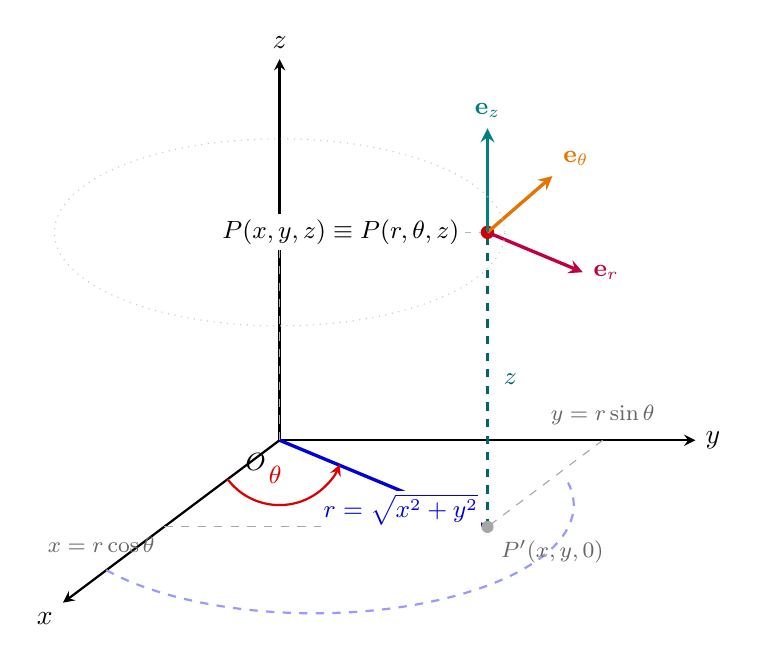
\begin{tikzpicture}[scale=1.1, >=stealth]
    % Coordinate axes
    \coordinate (O) at (0,0);
    \draw[->, thick] (O) -- (-2.5,-1.875) node[below left] {$x$};
    \draw[->, thick] (O) -- (4.8,0) node[right] {$y$};
    \draw[->, thick] (O) -- (0,4.4) node[above] {$z$};
    \node[below left=2pt, font=\small] at (O) {$O$};

    % Projection of P on xy-plane
    \coordinate (P_xy) at (2.4,-1.0);
    \coordinate (Px) at (-1.33,-1.0); % projection on x-axis
    \coordinate (Py) at (3.73,0);       % projection on y-axis

    % Point P in space at height z=2.4
    \coordinate (P) at (2.4,2.4);
    \coordinate (Pz) at (0,2.4);

    % Circular guide on xy-plane
    \draw[dashed, blue!40, thick] (-2.0,-1.5) arc (-143:12:3.0 and 1.25);

    % Grid lines on xy-plane
    \draw[dashed, gray!70] (Px) -- (P_xy);
    \draw[dashed, gray!70] (Py) -- (P_xy);
    \node[below left, font=\footnotesize, text=gray!80!black] at (Px) {$x=r\cos\theta$};
    \node[above=2pt, font=\footnotesize, text=gray!80!black] at (Py) {$y=r\sin\theta$};

    % Radial distance r on xy-plane
    \draw[-, very thick, blue!85!black] (O) -- (P_xy);
    \node[blue!85!black, font=\small, fill=white, inner sep=1pt] at (1.4,-0.8) {$r=\sqrt{x^2+y^2}$};

    % Angle theta arc
    \draw[->, thick, red!85!black] (-0.6,-0.45) arc (-143:-22:0.75);
    \node[red!85!black, font=\small] at (-0.05,-0.4) {$\theta$};

    % Height z line from P_xy to P
    \draw[dashed, very thick, teal!80!black] (P_xy) -- (P) node[midway, right=2pt, font=\small] {$z$};
    \draw[dashed, gray!60] (O) -- (Pz);
    \draw[dashed, gray!60] (Pz) -- (P);

    % Point P and P'
    \fill[gray!70] (P_xy) circle (2pt) node[below right=2pt, font=\footnotesize, text=gray!80!black] {$P'(x,y,0)$};
    \fill[red!80!black] (P) circle (2.2pt);
    \node[left=8pt, font=\small, fill=white, inner sep=2pt] at (P) {$P(x,y,z)\equiv P(r,\theta,z)$};

    % Orthogonal unit vectors at P
    \draw[->, very thick, purple] (P) -- ++(1.1,-0.46) node[right, font=\small] {$\mathbf{e}_r$};
    \draw[->, very thick, orange!90!black] (P) -- ++(0.75,0.65) node[above right, font=\small] {$\mathbf{e}_\theta$};
    \draw[->, very thick, teal] (P) -- ++(0,1.2) node[above, font=\small] {$\mathbf{e}_z$};

    % Cylinder surface ellipse outline at height z
    \draw[dotted, gray!45] (0,2.4) ellipse (2.6 and 1.08);
\end{tikzpicture}
\caption{直角坐标系 $(x,y,z)$ 与正交柱坐标系 $(r,\theta,z)$ 的几何变换示意图}\label{fig:cyl_transform}
\end{figure}
根据多元微积分复合函数的链式求导法则，两种坐标系下的偏微分算子满足如下关系：
\begin{equation}
\begin{bmatrix}
\dfrac{\partial}{\partial x} \\[10pt]
\dfrac{\partial}{\partial y} \\[10pt]
\dfrac{\partial}{\partial z}
\end{bmatrix}
=
\begin{bmatrix}
\dfrac{\partial r}{\partial x} & \dfrac{\partial\theta}{\partial x} & 0 \\[10pt]
\dfrac{\partial r}{\partial y} & \dfrac{\partial\theta}{\partial y} & 0 \\[10pt]
0 & 0 & 1
\end{bmatrix}
\begin{bmatrix}
\dfrac{\partial}{\partial r} \\[10pt]
\dfrac{\partial}{\partial\theta} \\[10pt]
\dfrac{\partial}{\partial z}
\end{bmatrix}
=
\begin{bmatrix}
\cos\theta & -\dfrac{\sin\theta}{r} & 0 \\[10pt]
\sin\theta & \dfrac{\cos\theta}{r} & 0 \\[10pt]
0 & 0 & 1
\end{bmatrix}
\begin{bmatrix}
\dfrac{\partial}{\partial r} \\[10pt]
\dfrac{\partial}{\partial\theta} \\[10pt]
\dfrac{\partial}{\partial z}
\end{bmatrix}.\label{eq:jacobi_transform}
\end{equation}
结合度规系数可知柱坐标下的 $\nabla$ 可以表示为：
\begin{align}
\nabla &= \frac{1}{h_r}\frac{\partial}{\partial r}\mathbf{e}_r + \frac{1}{h_\theta}\frac{\partial}{\partial\theta}\mathbf{e}_\theta + \frac{1}{h_z}\frac{\partial}{\partial z}\mathbf{e}_z \notag\\
&= \mathbf{e}_r\frac{\partial}{\partial r} + \mathbf{e}_\theta\frac1r\frac{\partial}{\partial\theta} + \mathbf{e}_z\frac{\partial}{\partial z}.\label{eq:grad_cyl}
\end{align}
对于矢量场 $\mathbf{A}$ 有柱坐标下的散度公式：
\begin{align}
\nabla\cdot\mathbf{A} &= \frac{1}{h_rh_\theta h_z}\left[\frac{\partial}{\partial r}(h_\theta h_zA_r) + \frac{\partial}{\partial\theta}(h_rh_zA_\theta) + \frac{\partial}{\partial z}(h_rh_\theta A_z)\right] \notag\\
&= \frac1r\frac{\partial}{\partial r}(rA_r) + \frac1r\frac{\partial A_\theta}{\partial\theta} + \frac{\partial A_z}{\partial z}.\label{eq:div_cyl}
\end{align}
使用\eqref{eq:grad_cyl}\eqref{eq:div_cyl}展开\eqref{eq:div_heat}和\eqref{eq:div_mass}得到：
\begin{align}
\nabla\cdot(k\nabla T) &= \frac1r\frac{\partial}{\partial r}\left(rk\frac{\partial T}{\partial r}\right) + \frac{1}{r^2}\frac{\partial}{\partial\theta}\left(k\frac{\partial T}{\partial\theta}\right) + \frac{\partial}{\partial z}\left(k\frac{\partial T}{\partial z}\right),\label{eq:div_heat_cyl}\\[10pt]
\nabla\cdot(D\nabla C) &= \frac1r\frac{\partial}{\partial r}\left(rD\frac{\partial C}{\partial r}\right) + \frac{1}{r^2}\frac{\partial}{\partial\theta}\left(D\frac{\partial C}{\partial\theta}\right) + \frac{\partial}{\partial z}\left(D\frac{\partial C}{\partial z}\right).\label{eq:div_mass_cyl}
\end{align}
得到柱坐标下的热质耦合方程如下：
\begin{align}
\rho c_p\frac{\partial T}{\partial t}
&=\frac1r\frac{\partial}{\partial r}\left(rk\frac{\partial T}{\partial r}\right)
+\frac{1}{r^2}\frac{\partial}{\partial\theta}\left(k\frac{\partial T}{\partial\theta}\right)
+\frac{\partial}{\partial z}\left(k\frac{\partial T}{\partial z}\right),\label{eq:cyl_heat}\\[10pt]
\frac{\partial C}{\partial t}
&=\frac1r\frac{\partial}{\partial r}\left(rD\frac{\partial C}{\partial r}\right)
+\frac{1}{r^2}\frac{\partial}{\partial\theta}\left(D\frac{\partial C}{\partial\theta}\right)
+\frac{\partial}{\partial z}\left(D\frac{\partial C}{\partial z}\right).\label{eq:cyl_mass}
\end{align}

\subsection{柱坐标扩散方程的简化}
式\eqref{eq:cyl_heat}与式\eqref{eq:cyl_mass}给出了柱坐标下的热质耦合方程。现在要对其进行近似简化，理由如下：
\begin{enumerate}[label=(\arabic*)]
  \item \textbf{旋转对称性}：
  已经假设药材外观呈规则圆柱体，并且质地均匀，具备严格的几何旋转对称性，以及烘房内热风流动平稳且均匀掠过圆柱外表面。环境温度 $T_a(t)$、环境水分浓度 $C_a(t)$ 以及表面对流换热与传质系数 $h, h_m$ 均不依赖于周向角 $\theta$。因此，温度场和水分场满足周向各向同性，即 $\frac{\partial T}{\partial\theta}=0$、$\frac{\partial C}{\partial\theta}=0$。

  \item \textbf{大长径比与大面积比}：
  药材实测几何尺寸为长度 $L=25\text{ cm}$，初始半径 $R_0=2\text{ cm}$（直径 $2R_0=4\text{ cm}$），长径比为 $L/(2R_0)=6.25\gg1$。圆柱周向侧面积为 $A_{\text{side}}=2\pi R_0 L$，而两端截面积之和仅为 $2A_{\text{end}}=2\pi R_0^2$。侧面积与端面积之比高达 $A_{\text{side}}/(2A_{\text{end}})=L/R_0=12.5$，这意味着超过 $92.6\%$ 的热量吸收与水分蒸发由侧表面承担，两端面通量占比极低，端部效应仅局限在极小的区域。

  \item \textbf{特征传递尺度与时间尺度}：
  热量由外周传入中心、水分的径向特征距离仅为半径 $R_0=2\text{ cm}$；而沿轴向传递的特征距离为半长 $L/2=12.5\text{ cm}$。由扩散的特征时间尺度准则 $\tau \sim l^2/D_{\text{eff}}$ 可知，轴向传递与径向传递特征时间之比为 $\tau_z/\tau_r \approx (L/2R_0)^2 = 6.25^2 \approx 39$ 倍。表明径向传递的速度远高于轴向，整个烘干过程中径向热质扩散占据绝对主导。

  \item \textbf{Biot数准则}：
  分别计算热传导与水分扩散的 Biot 数：
  \begin{align}
  Bi_T &= \frac{h R_0}{k} \approx \frac{25 \times 0.02}{0.36} \approx 1.39 > 0.1,\label{eq:biot_t}\\
  Bi_m &= \frac{h_m R_0}{D} \approx \frac{8.0\times 10^{-7} \times 0.02}{10^{-9}} \sim 16 \gg 0.1.\label{eq:biot_m}
  \end{align}
  在传热学与传质学准则中，当 $Bi > 0.1$ 时，介质内部的导热阻力与水分扩散阻力不可忽略，系统不能视为均质简化的集总参数模型，药材内部必定长期维持显著的径向温度梯度与水分梯度，即 $\frac{\partial T}{\partial r}\neq0$、$\frac{\partial C}{\partial r}\neq0$。
\end{enumerate}

\paragraph{小结}
依据上述四条证据，可以将三维柱坐标方程降维为一维，将证据单列如下：
\begin{enumerate}[label=(\arabic*)]
  \item \textbf{旋转对称性}：
  \begin{equation}
  \frac{\partial T}{\partial\theta} = 0,\qquad \frac{\partial C}{\partial\theta} = 0.\label{eq:theta_zero}
  \end{equation}
  \item \textbf{大长径比与大面积比}：
  \begin{equation}
  \left|\frac{\partial T}{\partial z}\right|\ll\left|\frac{\partial T}{\partial r}\right| \implies \frac{\partial T}{\partial z} \approx 0,\qquad
  \left|\frac{\partial C}{\partial z}\right|\ll\left|\frac{\partial C}{\partial r}\right| \implies \frac{\partial C}{\partial z} \approx 0.\label{eq:z_zero}
  \end{equation}
  \item \textbf{Biot数}：
  \begin{equation}
  Bi_T > 0.1 \implies \frac{\partial T}{\partial r} \neq 0,\qquad
  Bi_m \gg 0.1 \implies \frac{\partial C}{\partial r} \neq 0.\label{eq:r_nonzero}
  \end{equation}
\end{enumerate}

\paragraph{简化后的扩散方程}
于是，三维柱坐标控制方程\eqref{eq:cyl_heat}与\eqref{eq:cyl_mass}严格退化为一维径向非线性热质耦合方程。问题1--3在固定物理半径 $0\le r\le R$ 上满足：
\begin{align}
\rho(C)c_p(C)\frac{\partial T}{\partial t}
&=\frac1r\frac{\partial}{\partial r}\left(rk(C)\frac{\partial T}{\partial r}\right),\label{eq:heat}\\[10pt]
\frac{\partial C}{\partial t}
&=\frac1r\frac{\partial}{\partial r}\left(rD(C,T)\frac{\partial C}{\partial r}\right).\label{eq:mass}
\end{align}

\subsection{边界条件}
为了求解这个偏微分方程，还需要确定几组边界条件：
\begin{enumerate}[label=(\arabic*)]
  \item \textbf{圆柱中心对称条件}：
  在药材中心轴线 $r=0$ 处，由于具备中心对称性，温度场与水分场关于轴心线呈镜像对称，于是径向梯度必恒等于零：
  \begin{equation}
  \left.\frac{\partial T}{\partial r}\right|_{r=0} = 0,\qquad \left.\frac{\partial C}{\partial r}\right|_{r=0} = 0.\label{eq:centerbc}
  \end{equation}

  \item \textbf{外表面 Robin 传热与传质条件}：
  在药材与烘房热风接触的侧表面 $r=R$ 处，传热与传质遵循界面通量守恒原理。药材由内向外的热通量与水分通量，等于表面向外部环境对流换热与对流蒸发传质的净通量，分别服从 Newton 冷却定律与表面对流传质定律：
  \begin{align}
  -k(C_s)\left.\frac{\partial T}{\partial r}\right|_{r=R} &= h\left[T(R,t)-T_a(t)\right],\label{eq:robin_t}\\[8pt]
  -D(C_s,T_s)\left.\frac{\partial C}{\partial r}\right|_{r=R} &= h_m\left[C(R,t)-C_a(t)\right],\label{eq:robin_m}
  \end{align}
  其中 $T_s = T(R,t)$ 与 $C_s = C(R,t)$ 分别表示药材外表面的温度与干基含水率，$T_a(t)$ 与 $C_a(t)$ 分别为由附件1给出的时变烘房空气温度与水分浓度。
\end{enumerate}

\paragraph{总结}
综合简化后的扩散方程与边界定解条件，问题1--3在 $0\le r\le R$ 下构成的热质耦合方程组可统一表示为：
\begin{equation}
\begin{cases}
\rho(C)c_p(C)\dfrac{\partial T}{\partial t} = \dfrac{1}{r}\dfrac{\partial}{\partial r}\left(rk(C)\dfrac{\partial T}{\partial r}\right),\\[12pt]
\dfrac{\partial C}{\partial t} = \dfrac{1}{r}\dfrac{\partial}{\partial r}\left(rD(C,T)\dfrac{\partial C}{\partial r}\right),\\[12pt]
\left.\dfrac{\partial T}{\partial r}\right|_{r=0} = 0,\quad \left.\dfrac{\partial C}{\partial r}\right|_{r=0} = 0,\\[12pt]
-k(C_s)\left.\dfrac{\partial T}{\partial r}\right|_{r=R} = h\left[T(R,t)-T_a(t)\right],\\[12pt]
-D(C_s,T_s)\left.\dfrac{\partial C}{\partial r}\right|_{r=R} = h_m\left[C(R,t)-C_a(t)\right].
\end{cases}\label{eq:coupled_system}
\end{equation}
针对具体求解，将式\eqref{eq:coupled_system}分别与各问对应附录中的物性参数联立即可。

\section{问题求解}

\subsection{问题1：恒定物性下的初期瞬态场}

\subsubsection{求解思路与联立方程}
问题1采用附录2给出的恒定热物性，并保留含水率对扩散系数的影响。令
\begin{equation}
\begin{aligned}
\rho_1&=820\ \mathrm{kg/m^3},&
c_{p1}&=2600\ \mathrm{J/(kg\cdot K)},\\
k_1&=0.36\ \mathrm{W/(m\cdot K)},&
D_1(C)&=7.0\times10^{-9}\exp\!\left(-\frac{0.89}{C}\right)\ \mathrm{m^2/s}.
\end{aligned}
\end{equation}
将上述物性与附件1的环境温湿度边界代入第五章模型，得到
\begin{equation}
\left\{
\begin{aligned}
\rho_1c_{p1}\frac{\partial T}{\partial t}
&=\frac{1}{r}\frac{\partial}{\partial r}\!\left(rk_1\frac{\partial T}{\partial r}\right),\\
\frac{\partial C}{\partial t}
&=\frac{1}{r}\frac{\partial}{\partial r}\!\left(rD_1(C)\frac{\partial C}{\partial r}\right),\\
\left.\frac{\partial T}{\partial r}\right|_{r=0}
&=\left.\frac{\partial C}{\partial r}\right|_{r=0}=0,\\
-k_1\left.\frac{\partial T}{\partial r}\right|_{r=R}
&=h[T(R,t)-T_a(t)],\\
-D_1(C_s)\left.\frac{\partial C}{\partial r}\right|_{r=R}
&=h_m[C(R,t)-C_a(t)],\\
T(r,0)&=301.15\ \mathrm{K},\qquad C(r,0)=2.55,
\end{aligned}
\right.\label{eq:q1_system}
\end{equation}
其中 $R=0.02\ \mathrm{m}$、$h=25\ \mathrm{W/(m^2\cdot K)}$、
$h_m=8.0\times10^{-7}\ \mathrm{m/s}$。由此可直接计算前30 min内的温湿场。

\subsubsection{数值求解}
为兼顾守恒性与计算效率，仅对空间变量作有限体积离散。令
$(\phi,q,\Gamma)=(T,\rho c_p,k)$ 或 $(C,1,D)$，在网格
$r_i=i\Delta r$ 上对控制体积分，内部节点满足
\begin{equation}
q_i\omega_i^r\frac{d\phi_i}{dt}=F_{i+1/2}-F_{i-1/2},\qquad
F_{i+1/2}=r_{i+1/2}\Gamma_{i+1/2}
\frac{\phi_{i+1}-\phi_i}{\Delta r},\label{eq:fvm-r}
\end{equation}
其中 $\omega_i^r=(r_{i+1/2}^2-r_{i-1/2}^2)/2$，界面系数取调和平均
$\Gamma_{i+1/2}=2\Gamma_i\Gamma_{i+1}/(\Gamma_i+\Gamma_{i+1})$
\cite{patankar}。圆心通量取零，外表面 Robin 条件直接写成
\begin{equation}
F_R^T=Rh(T_a-T_N),\qquad F_R^C=Rh_m(C_a-C_N).
\end{equation}
内部通量相消后，离散总水分 $M_h=2\pi\sum_i\omega_i^rC_i$ 满足
\begin{equation}
\frac{dM_h}{dt}=2\pi F_R^C=-2\pi Rh_m(C_N-C_a),
\label{eq:global_conservation}
\end{equation}
说明水分变化仅由表面对流传质引起。

将各节点的温度、含水率依次排列为状态向量，PDE 即化为标准初值问题
\begin{equation}
\mathbf y=[T_0,\ldots,T_N,C_0,\ldots,C_N]^T,\qquad
\frac{d\mathbf y}{dt}=\mathbf F(t,\mathbf y),\quad \mathbf y(0)=\mathbf y_0.
\label{eq:ode_standard}
\end{equation}
由于扩散模态时间尺度相差较大，采用隐式 BDF 方法。其 $k$ 阶格式可写为
\begin{equation}
\sum_{j=0}^{k}\alpha_j\mathbf y_{n+1-j}
=\Delta t_n\beta\,\mathbf F(t_{n+1},\mathbf y_{n+1}),\qquad 1\le k\le5,
\end{equation}
每一步通过 Newton 迭代求解，并按局部误差自适应调整步长与阶次
\cite{hairer}。程序中将有限体积组装得到的右端函数直接传入求解器，关键调用如下：
\begin{lstlisting}[caption={有限体积右端项传入 BDF 求解器的关键代码},label={code:solver}]
grid, rhs = make_fixed_rhs(R, node_count, model, environment)
y0 = np.r_[np.full(node_count, T0), np.full(node_count, C0)]
sol = solve_ivp(
    rhs, (0.0, t_end), y0, method="BDF",
    rtol=1e-6, atol=1e-8, max_step=300.0,
    jac_sparsity=coupled_jacobian_sparsity(node_count),
    events=events,
)
\end{lstlisting}
其中相对、绝对误差限分别为 $10^{-6}$ 和 $10^{-8}$，并利用块带状雅可比稀疏结构加速计算。求解器的循环过程如图\ref{fig:flowchart}所示。
\begin{figure}[H]
\centering
\begin{tikzpicture}[
    font=\footnotesize,
    process/.style={
        rectangle, rounded corners=2.5pt,
        minimum width=4.2cm, minimum height=0.54cm,
        align=center, draw=blue!60!black, fill=blue!4, thick
    },
    decision/.style={
        diamond, aspect=2.25,
        minimum width=2.8cm, minimum height=0.68cm,
        align=center, draw=orange!75!black, fill=orange!7, thick
    },
    adjust/.style={
        rectangle, rounded corners=2.5pt,
        minimum width=2.6cm, minimum height=0.52cm,
        align=center, draw=teal!65!black, fill=teal!5, thick
    },
    arrow/.style={-{Stealth[length=2.0mm]}, thick, color=black!70}
]
\node (init) [process] {输入与网格};
\node (fvm) [process, below=0.25cm of init] {FVM 组装};
\node (bdf) [process, below=0.25cm of fvm] {BDF 试步};
\node (error) [decision, below=0.38cm of bdf] {误差通过？};
\node (adjust) [adjust, right=1.55cm of error] {调步长/阶次};
\node (event) [decision, below=0.48cm of error] {$g(t)\le 0$？};
\node (out) [process, below=0.42cm of event] {60 s 校核与输出};
\draw [arrow] (init)--(fvm);
\draw [arrow] (fvm)--(bdf);
\draw [arrow] (bdf)--(error);
\draw [arrow] (error)--node[left] {是} (event);
\draw [arrow] (error.east)--node[above] {否} (adjust.west);
\draw [arrow] (adjust.north)|-(bdf.east);
\draw [arrow] (event)--node[left] {是} (out);
\draw [arrow] (event.west)--++(-1.25,0)|-node[pos=0.25,left] {否：下一步} (bdf.west);
\end{tikzpicture}
\caption{FVM--BDF 自适应循环求解流程}\label{fig:flowchart}
\end{figure}

\subsubsection{计算结果}
采用161个径向节点计算至1800 s。此时中心、表面温度分别为
33.5754 $^\circ$C 和 36.7859 $^\circ$C；中心含水率仍为
2.5500 kg/kg，表面已降至 1.5103 kg/kg。温度由表面向内传导，水分则先在外层形成低含水率边界层，结果见图\ref{fig:q1_profiles}和图\ref{fig:q1_heatmaps}。
\begin{figure}[H]
\centering
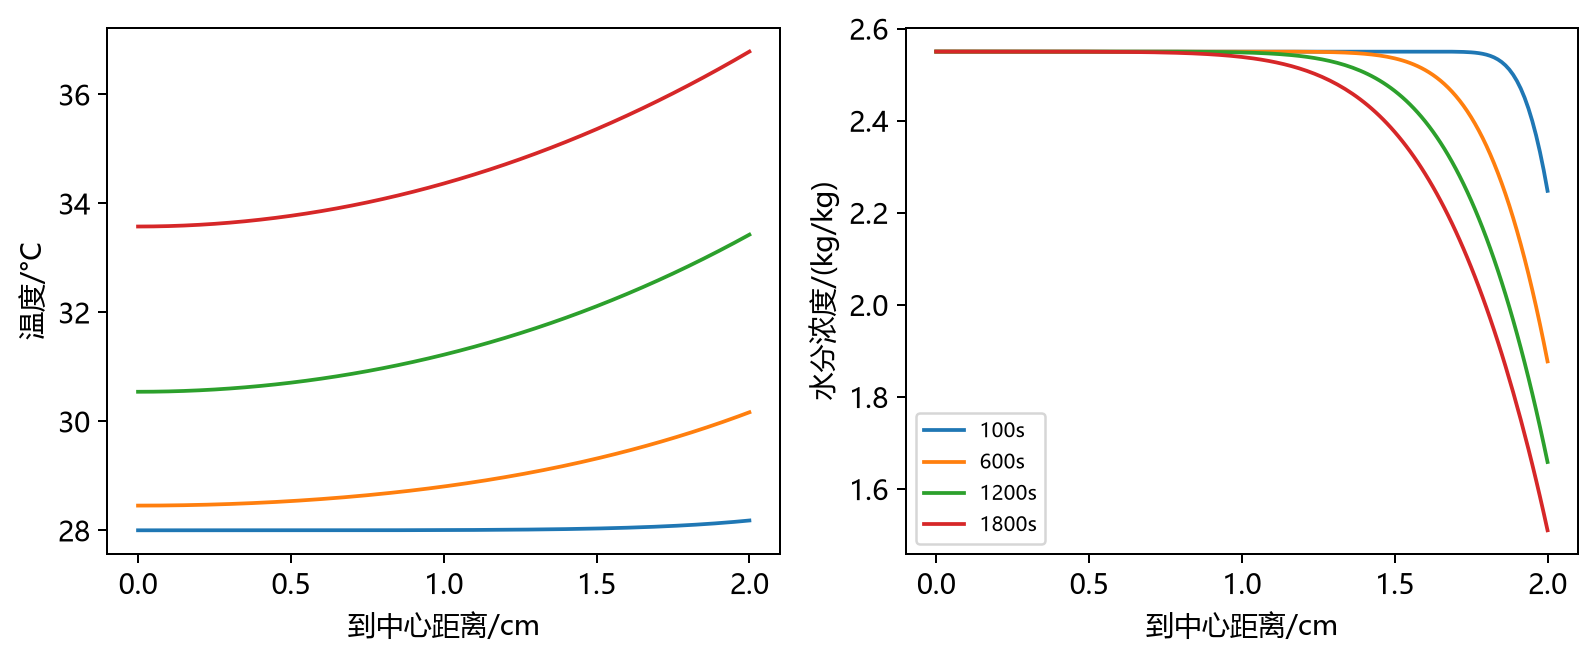
\includegraphics[width=0.88\textwidth]{question1_profiles.png}
\caption{问题1在不同代表时刻的径向温度与水分浓度分布剖面}\label{fig:q1_profiles}
\end{figure}
\begin{figure}[H]
\centering
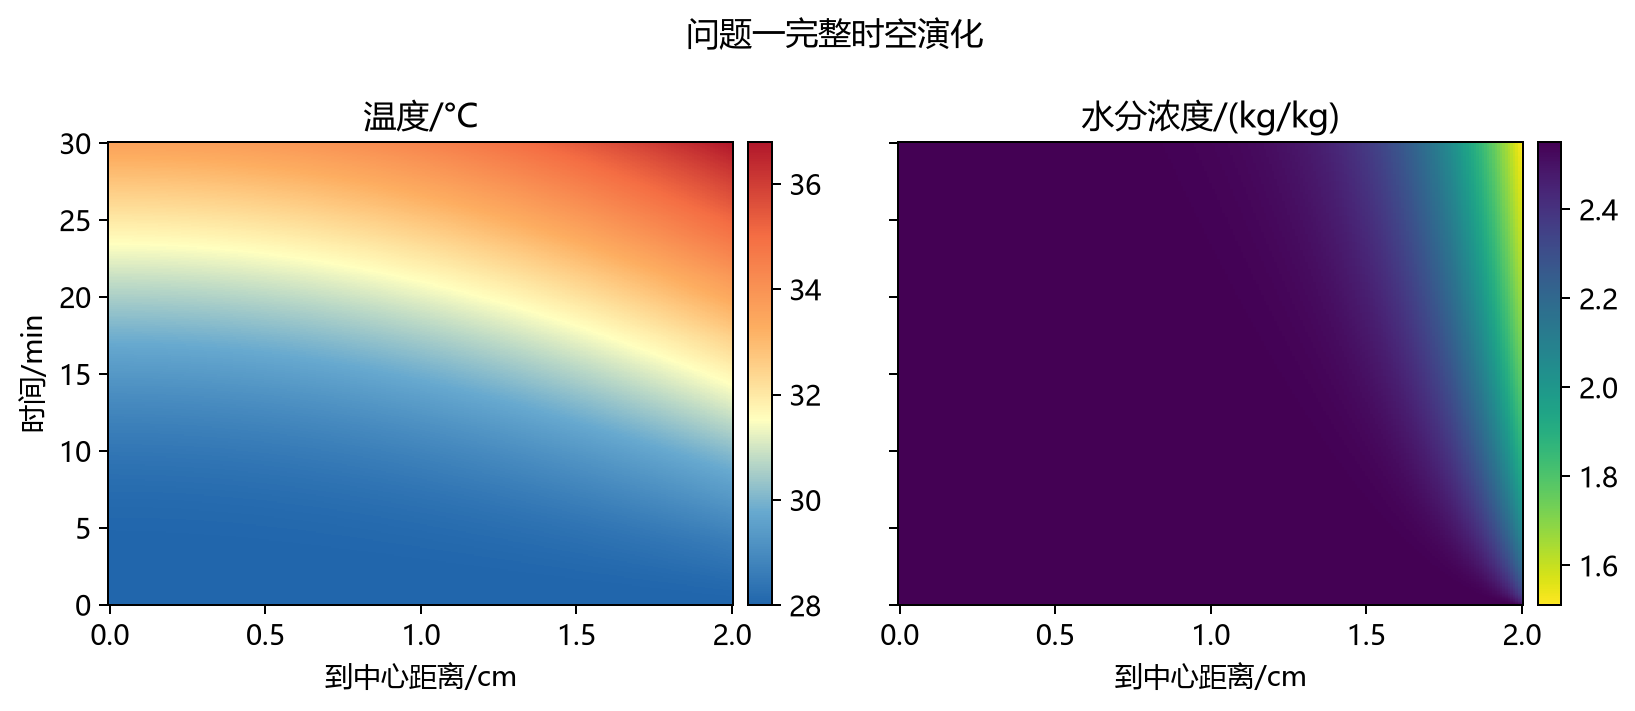
\includegraphics[width=0.92\textwidth]{question1_heatmaps.png}
\caption{问题1前30 min温度场与水分场的二维时空全景演化热力图}\label{fig:q1_heatmaps}
\end{figure}

\subsection{问题2：非线性物性下的耦合演化}

\subsubsection{求解思路与联立方程}
问题2沿用式\eqref{eq:q1_system}的控制方程、初始条件和边界条件，仅将物性替换为附录3给出的非线性函数：
\begin{equation}
\begin{aligned}
\rho_2(C)&=650+128C,\\
c_{p2}(C)&=1450+2736\frac{C}{C+1},\\
k_2(C)&=0.21+0.38\frac{C}{C+1},\\
D_2(C,T)&=2.4\times10^{-3}
\exp\!\left(-\frac{0.45}{C}\right)
\exp\!\left(-\frac{3850}{T}\right).
\end{aligned}\label{eq:q2_properties}
\end{equation}
将式\eqref{eq:q2_properties}代入传热传质方程即得到问题2的联立系统；按与问题1相同的有限体积--BDF流程，采用201个径向节点求解前3 h。

\subsubsection{计算结果}
在10800 s时，中心与表面温度分别为49.8484 $^\circ$C和49.8975 $^\circ$C，温差不足0.05 $^\circ$C；中心与表面含水率分别为1.7658 kg/kg和1.0080 kg/kg。说明温度场已接近准平衡，而水分场仍保持明显梯度，结果见图\ref{fig:q2_profiles}和图\ref{fig:q2_heatmaps}。
\begin{figure}[H]
\centering
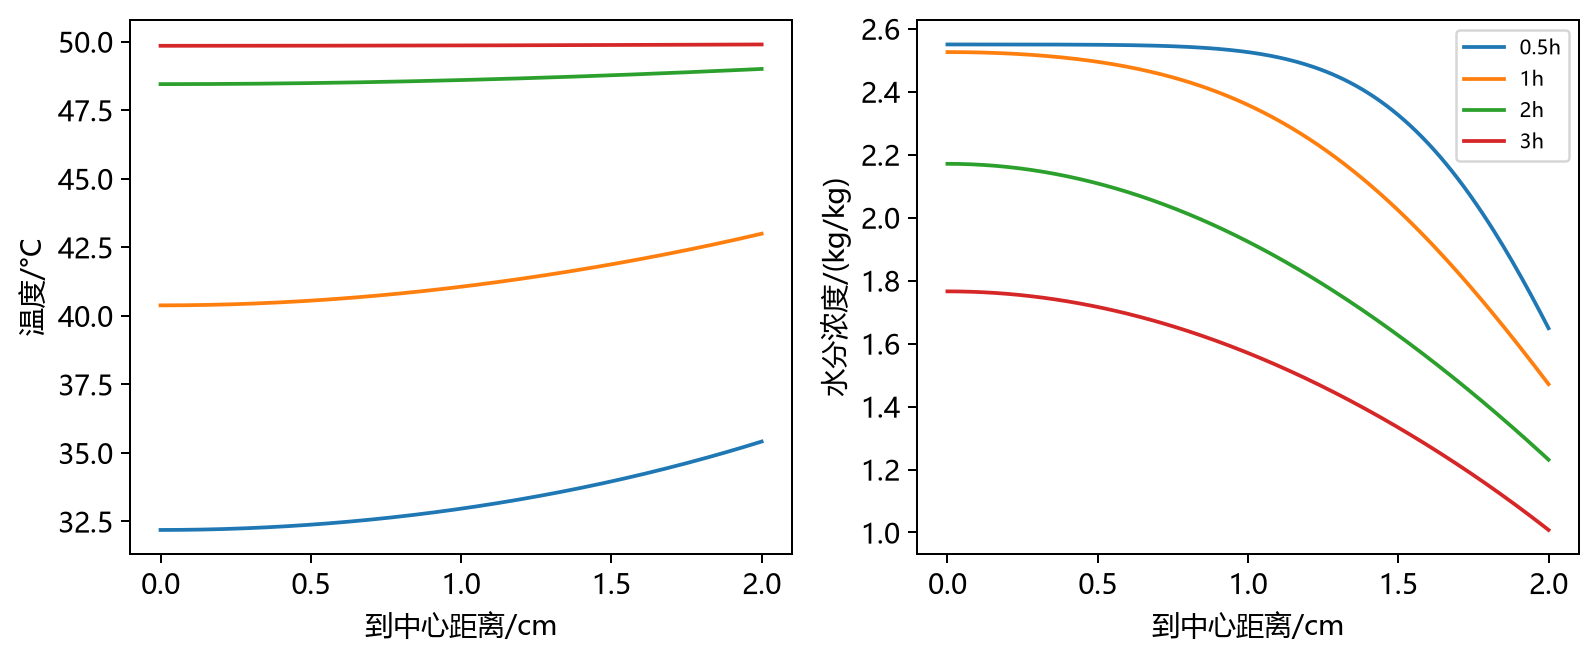
\includegraphics[width=0.88\textwidth]{question2_profiles.png}
\caption{问题2在代表时刻的径向温度与水分浓度分布剖面}\label{fig:q2_profiles}
\end{figure}
\begin{figure}[H]
\centering
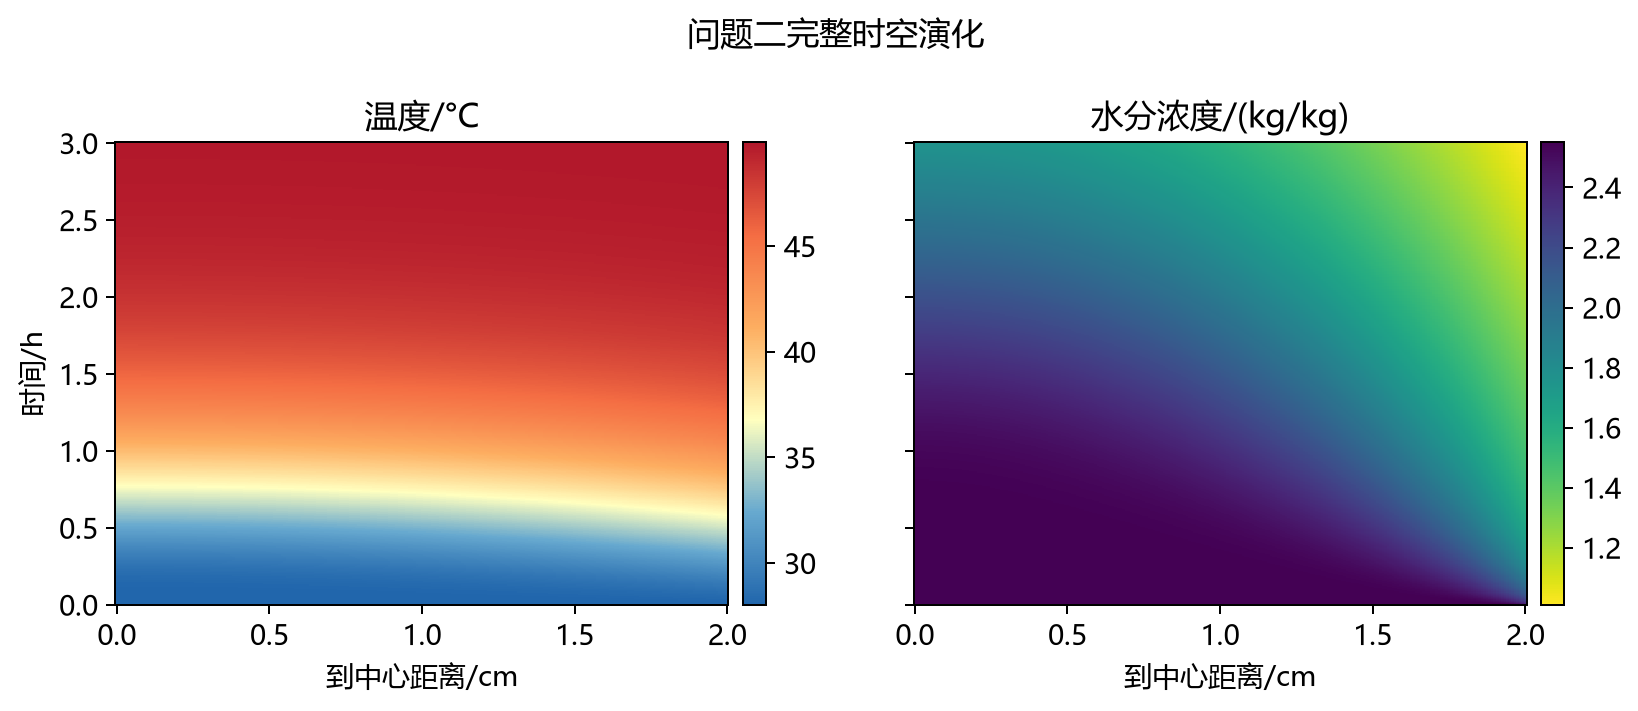
\includegraphics[width=0.92\textwidth]{question2_heatmaps.png}
\caption{问题2前3 h温度场与水分场的二维时空全景演化热力图}\label{fig:q2_heatmaps}
\end{figure}

\subsection{问题3：固定半径下的干燥终点}

\subsubsection{求解思路与联立方程}
问题3直接沿用问题2的联立系统，将计算时域延长并增加全场终止事件
\begin{equation}
g(t)=\max_{0\le r\le R}C(r,t)-0.15=0.
\label{eq:q3_event}
\end{equation}
采用801个径向节点连续定位理论终点，再在60 s输出网格上取首个满足
$\max C<0.15$ 的安全时刻。

\subsubsection{计算结果}
连续临界时刻为57.5685 h；60 s网格上的安全达标时刻为
\begin{equation}
\boxed{t_3=207300\ \mathrm{s}=\QThreeDryHours\ \mathrm{h}\approx2.40\ \mathrm{d}}.
\end{equation}
此时全域最大含水率为0.149984。表面在12.55 h即达到0.15，而中心需57.58 h，表明内部扩散是终点控制环节，故采用全场最大值判停。计算结果见图\ref{fig:drying}和图\ref{fig:q3_heatmaps}。
\begin{figure}[H]
\centering
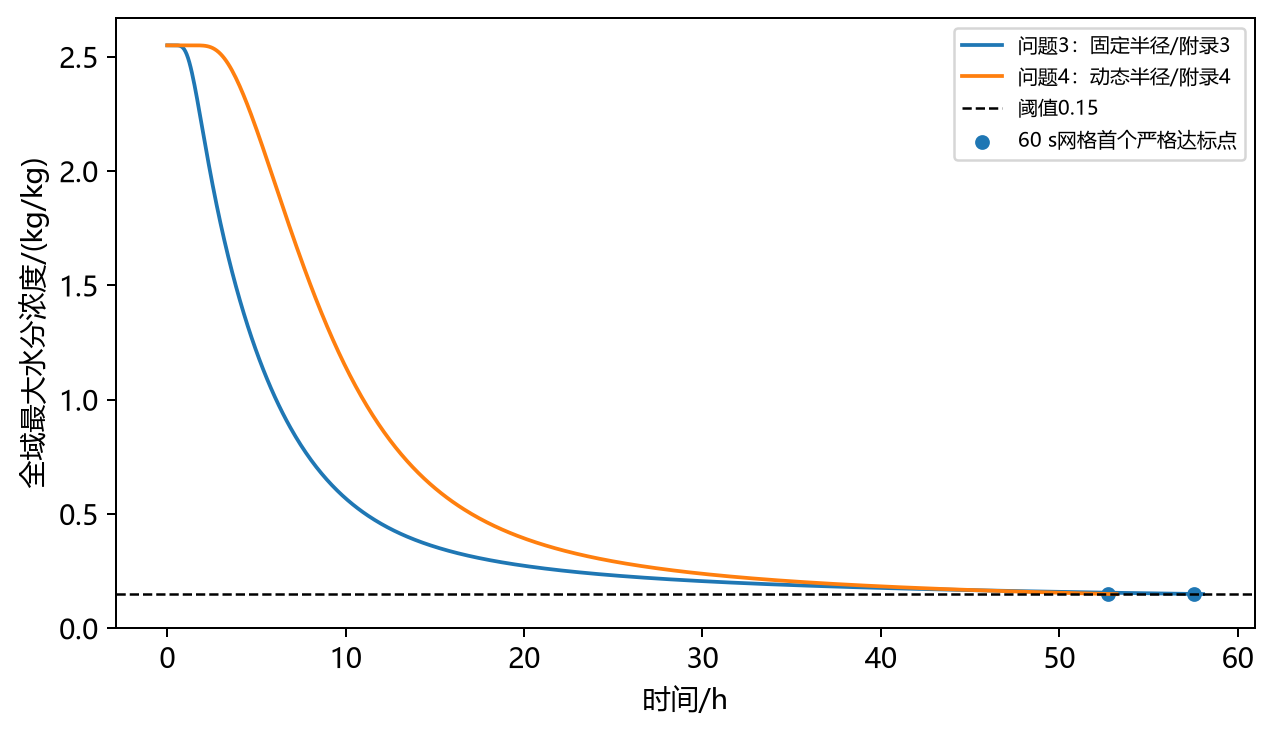
\includegraphics[width=0.82\textwidth]{drying_threshold.png}
\caption{问题3与问题4全域最大水分浓度随时间演化曲线及60 s达标点定位}\label{fig:drying}
\end{figure}
\begin{figure}[H]
\centering
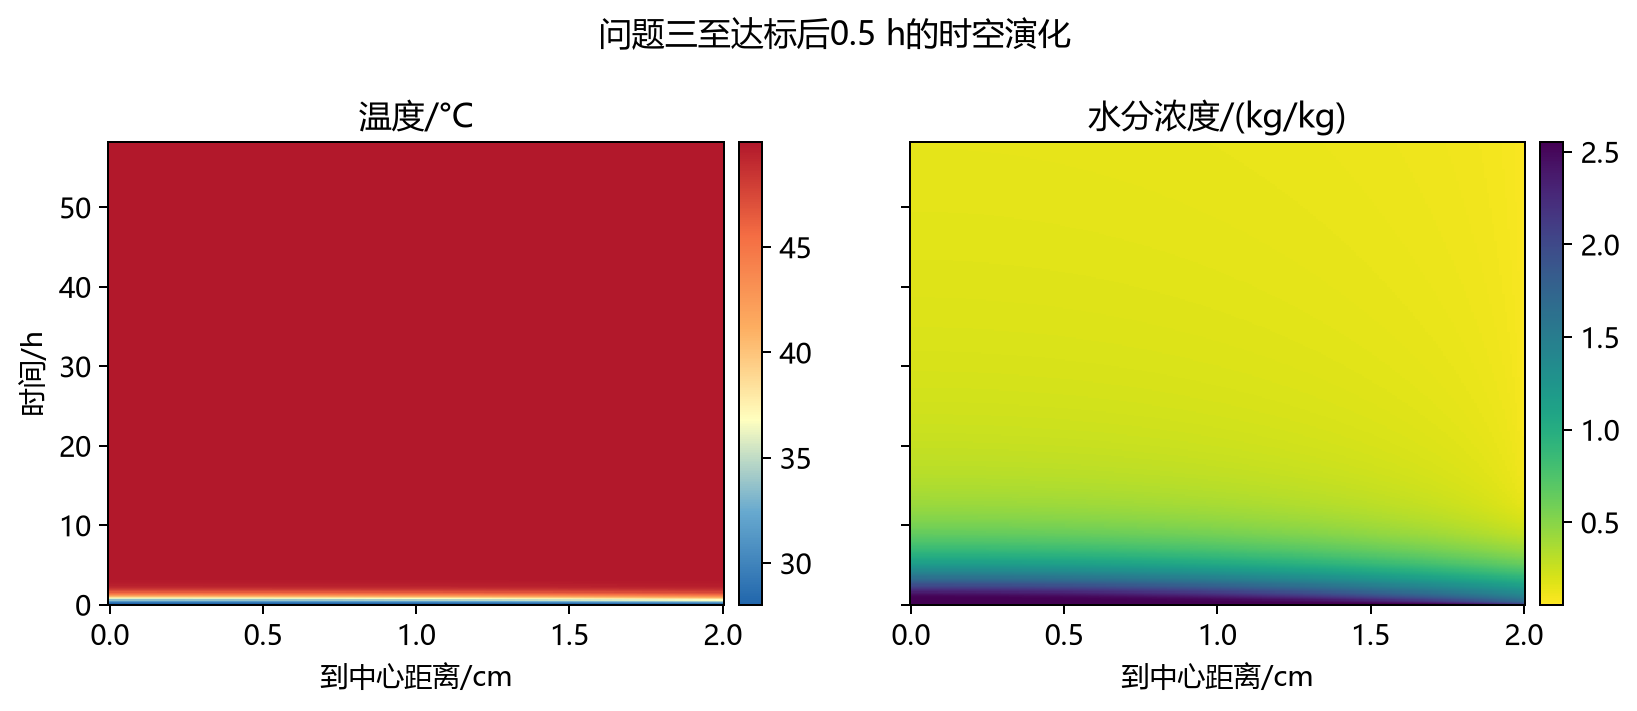
\includegraphics[width=0.92\textwidth]{question3_heatmaps.png}
\caption{问题3直至达标后0.5 h的温度场与水分场二维时空演化热力图}\label{fig:q3_heatmaps}
\end{figure}

\subsection{问题4：收缩域下的干燥终点}

\subsubsection{求解思路与联立方程}
问题4采用附录4的物性函数
\begin{equation}
\begin{aligned}
\rho_4(C)&=760+90C,\\
c_{p4}(C)&=1850+2150\frac{C}{C+1},\\
k_4(C)&=0.12+0.20\frac{C}{C+1},\\
D_4(C,T)&=4.2\times10^{-4}
\exp\!\left(-\frac{0.30}{C}\right)
\exp\!\left(-\frac{3850}{T}\right).
\end{aligned}\label{eq:q4_properties}
\end{equation}
同时半径按附件2数据随时间收缩。为避免移动网格，引入相对坐标
\begin{equation}
\xi=\frac{r}{R(t)},\qquad 0\le\xi\le1,
\end{equation}
并在相邻测量点 $(t_j,R_j)$ 间令
\begin{equation}
R(t)=R_j+\frac{R_{j+1}-R_j}{t_{j+1}-t_j}(t-t_j),\qquad
\dot R(t)=\frac{R_{j+1}-R_j}{t_{j+1}-t_j}.
\end{equation}
由
$\left.\partial_t\phi\right|_r=\left.\partial_t\phi\right|_\xi-
\xi(\dot R/R)\partial_\xi\phi$ 和
$\partial_r=R^{-1}\partial_\xi$，原方程化为固定域上的联立系统
\begin{align}
\frac{\partial T}{\partial t}
&=\xi\frac{\dot R}{R}\frac{\partial T}{\partial\xi}
+\frac{1}{\rho_4c_{p4}R^2\xi}
\frac{\partial}{\partial\xi}\!\left(\xi k_4\frac{\partial T}{\partial\xi}\right),
\label{eq:movingT}\\
\frac{\partial C}{\partial t}
&=\xi\frac{\dot R}{R}\frac{\partial C}{\partial\xi}
+\frac{1}{R^2\xi}
\frac{\partial}{\partial\xi}\!\left(\xi D_4\frac{\partial C}{\partial\xi}\right).
\label{eq:movingC}
\end{align}
在 $\xi=0$ 处取对称边界，在 $\xi=1$ 处联立
\begin{equation}
-\frac{k_4}{R}\frac{\partial T}{\partial\xi}=h(T_s-T_a),\qquad
-\frac{D_4}{R}\frac{\partial C}{\partial\xi}=h_m(C_s-C_a),
\end{equation}
并沿用式\eqref{eq:q3_event}的终止条件。采用601个相对坐标节点，以同一有限体积--BDF流程求解；与前三问相比仅增加了收缩引起的几何输运项。

\subsubsection{计算结果}
连续临界时刻为52.7135 h；60 s输出网格上的安全达标时刻及对应半径为
\begin{equation}
\boxed{t_4=189780\ \mathrm{s}=\QFourDryHours\ \mathrm{h}\approx2.20\ \mathrm{d}},
\qquad R(t_4)=\QFourDryRadius\ \mathrm{cm}.
\end{equation}
此时全域最大含水率为0.149994。固定物理采样点若满足 $r_j>R(t)$，则已位于收缩后的外部空气域，按题意在表格中留空；“药材表面”列始终取 $\xi=1$ 处的值。结果见图\ref{fig:q4_heatmaps}，机理对照见第\ref{sec:mechanism_decoupling}节。
\begin{figure}[H]
\centering
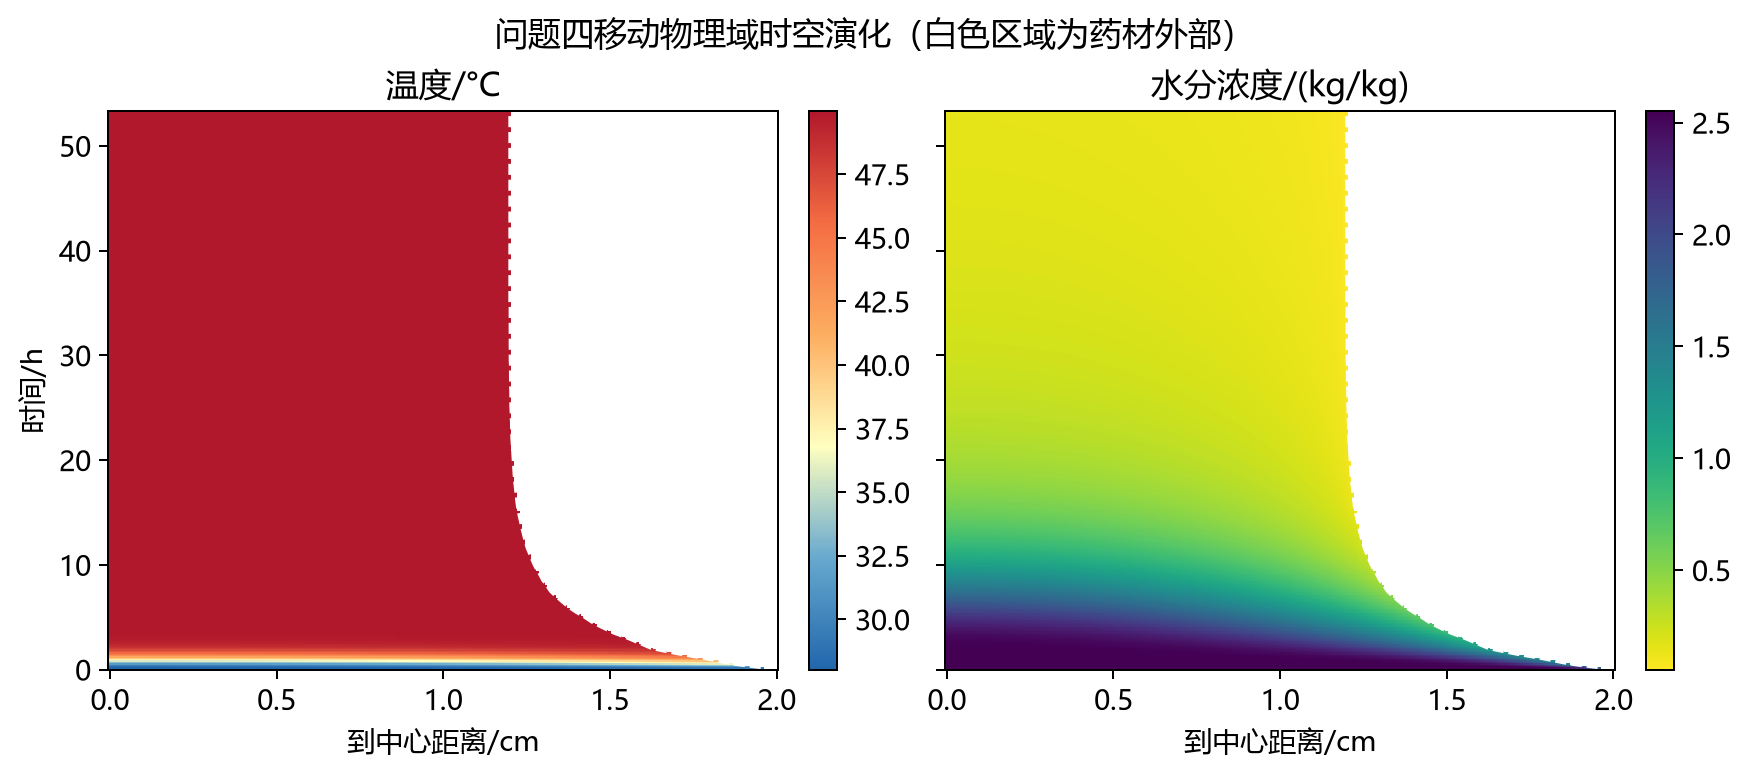
\includegraphics[width=0.92\textwidth]{question4_heatmaps.png}
\caption{问题4移动物理域温湿场时空演化热力图（白色区域为药材收缩后的外部空间）}\label{fig:q4_heatmaps}
\end{figure}

\subsection{题目规定的标准输出报表}
将精细计算网格投影到题目规定的空间采样位置（$0\sim2\ \mathrm{cm}$，步长$0.1\ \mathrm{cm}$），所得六组结果如下；完整电子表格见支撑材料。
\begin{table}[H]
\centering
\caption{问题1：30 min 内药材温度（$^\circ$C）}\label{tab:q1t}
\small
\begin{tabular}{rrrrrr}
\toprule
时间/s & 0 cm & 0.5 cm & 1.0 cm & 1.5 cm & 2.0 cm \\
\midrule
100 & 28.0001 & 28.0003 & 28.0041 & 28.0327 & 28.1801 \\
300 & 28.0408 & 28.0635 & 28.1514 & 28.3681 & 28.8489 \\
600 & 28.4533 & 28.5360 & 28.8039 & 29.3159 & 30.1652 \\
900 & 29.3243 & 29.4583 & 29.8755 & 30.6161 & 31.7304 \\
1200 & 30.5427 & 30.7098 & 31.2223 & 32.1126 & 33.4276 \\
1500 & 31.9957 & 32.1867 & 32.7660 & 33.7463 & 35.1203 \\
1800 & 33.5753 & 33.7720 & 34.3642 & 35.3621 & 36.7856 \\
\bottomrule
\end{tabular}
\end{table}

\begin{table}[H]
\centering
\caption{问题1：30 min 内水分浓度（kg/kg）}\label{tab:q1c}
\small
\begin{tabular}{rrrrrr}
\toprule
时间/s & 0 cm & 0.5 cm & 1.0 cm & 1.5 cm & 2.0 cm \\
\midrule
100 & 2.5500 & 2.5500 & 2.5500 & 2.5500 & 2.2471 \\
300 & 2.5500 & 2.5500 & 2.5500 & 2.5492 & 2.0508 \\
600 & 2.5500 & 2.5500 & 2.5500 & 2.5353 & 1.8770 \\
900 & 2.5500 & 2.5500 & 2.5497 & 2.5045 & 1.7547 \\
1200 & 2.5500 & 2.5500 & 2.5482 & 2.4646 & 1.6586 \\
1500 & 2.5500 & 2.5499 & 2.5445 & 2.4206 & 1.5787 \\
1800 & 2.5500 & 2.5497 & 2.5383 & 2.3755 & 1.5102 \\
\bottomrule
\end{tabular}
\end{table}

\begin{table}[H]
\centering
\caption{问题2：3 h 内药材温度（$^\circ$C）}\label{tab:q2t}
\small
\begin{tabular}{rrrrrr}
\toprule
时间/h & 0 cm & 0.5 cm & 1.0 cm & 1.5 cm & 2.0 cm \\
\midrule
0.5 & 32.1892 & 32.3821 & 32.9659 & 33.9608 & 35.4130 \\
1.0 & 40.3816 & 40.5536 & 41.0605 & 41.8782 & 42.9976 \\
1.5 & 45.8468 & 45.9348 & 46.1930 & 46.6051 & 47.1401 \\
2.0 & 48.4502 & 48.4881 & 48.5984 & 48.7736 & 49.0033 \\
2.5 & 49.4670 & 49.4792 & 49.5137 & 49.5653 & 49.6609 \\
3.0 & 49.8495 & 49.8553 & 49.8746 & 49.9101 & 49.9664 \\
\bottomrule
\end{tabular}
\end{table}

\begin{table}[H]
\centering
\caption{问题2：3 h 内水分浓度（kg/kg）}\label{tab:q2c}
\small
\begin{tabular}{rrrrrr}
\toprule
时间/h & 0 cm & 0.5 cm & 1.0 cm & 1.5 cm & 2.0 cm \\
\midrule
0.5 & 2.5499 & 2.5489 & 2.5256 & 2.3257 & 1.6486 \\
1.0 & 2.5257 & 2.4948 & 2.3578 & 2.0230 & 1.4711 \\
1.5 & 2.3861 & 2.3256 & 2.1344 & 1.8020 & 1.3476 \\
2.0 & 2.1709 & 2.1084 & 1.9236 & 1.6259 & 1.2311 \\
2.5 & 1.9566 & 1.9006 & 1.7360 & 1.4720 & 1.1166 \\
3.0 & 1.7662 & 1.7165 & 1.5702 & 1.3333 & 1.0081 \\
\bottomrule
\end{tabular}
\end{table}

\begin{longtable}{rrrrrr}
\caption{问题3每6 h及达标时刻的水分浓度}\label{tab:q3}\\
\toprule
时间/h & 0 cm & 0.5 cm & 1.0 cm & 1.5 cm & 2.0 cm \\
\midrule
\endfirsthead
\toprule
时间/h & 0 cm & 0.5 cm & 1.0 cm & 1.5 cm & 2.0 cm \\
\midrule
\endhead
6 & 1.0169 & 0.9881 & 0.9015 & 0.7550 & 0.5328 \\
12 & 0.4561 & 0.4431 & 0.4030 & 0.3297 & 0.1642 \\
18 & 0.2988 & 0.2915 & 0.2687 & 0.2253 & 0.0844 \\
24 & 0.2378 & 0.2327 & 0.2167 & 0.1856 & 0.0664 \\
30 & 0.2058 & 0.2019 & 0.1892 & 0.1642 & 0.0598 \\
36 & 0.1859 & 0.1826 & 0.1719 & 0.1505 & 0.0566 \\
42 & 0.1721 & 0.1692 & 0.1598 & 0.1408 & 0.0548 \\
48 & 0.1619 & 0.1592 & 0.1508 & 0.1336 & 0.0537 \\
54 & 0.1539 & 0.1515 & 0.1437 & 0.1278 & 0.0530 \\
57.5303 & 0.1500 & 0.1477 & 0.1402 & 0.1250 & 0.0527 \\
\bottomrule
\end{longtable}

\begin{longtable}{rrrrrr}
\caption{问题4每6 h及达标时刻的水分浓度}\label{tab:q4}\\
\toprule
时间/h & 半径/cm & 0 cm & 0.5 cm & 1.0 cm & 药材表面 \\
\midrule
\endfirsthead
\toprule
时间/h & 半径/cm & 0 cm & 0.5 cm & 1.0 cm & 药材表面 \\
\midrule
\endhead
6 & 1.3740 & 1.9530 & 1.7835 & 1.2579 & 0.5678 \\
12 & 1.2480 & 0.8738 & 0.7767 & 0.4862 & 0.2147 \\
18 & 1.2140 & 0.4594 & 0.4131 & 0.2653 & 0.1021 \\
24 & 1.2040 & 0.3072 & 0.2806 & 0.1903 & 0.0714 \\
30 & 1.2010 & 0.2381 & 0.2199 & 0.1556 & 0.0610 \\
36 & 1.2000 & 0.2000 & 0.1861 & 0.1357 & 0.0567 \\
42 & 1.2000 & 0.1761 & 0.1648 & 0.1228 & 0.0545 \\
48 & 1.2000 & 0.1597 & 0.1500 & 0.1136 & 0.0533 \\
52.6776 & 1.2000 & 0.1500 & 0.1413 & 0.1081 & 0.0526 \\
\bottomrule
\end{longtable}



\section{模型检验、机理探讨与拓展评价}

\subsection{数值算法可靠性}
随着径向网格的逐步加密，各问计算结果单调收敛至高精度数值极限。问题3将径向网格由 401 节点逐步加密至 801 节点与 1201 节点，干燥时长由 57.75 h 收敛至 57.57 h 与 57.54 h，加密相对变化仅为 \QThreeGridChange；问题4由 321 节点加密至 601 节点与 801 节点，时长高度稳定在 52.71 h，相对变化仅为 \QFourGridChange。具体网格测试数据汇总于表\ref{tab:grid}，充分证明正式计算所选取的网格密度已完全处于渐近网格无关区。

\begin{table}[H]
\centering
\caption{干燥时长的空间网格收敛数据汇总}\label{tab:grid}
\begin{tabular}{rrr@{\hspace{2.5em}}rrr}
\toprule
\multicolumn{3}{c}{问题3：划分物理半径 $r$} & \multicolumn{3}{c}{问题4：划分相对坐标 $\xi$}\\
节点数 & 空间步长 $\Delta r$/cm & 达标时长/h & 节点数 & 初始间距/cm & 达标时长/h\\
\midrule
401  & 0.005000 & 57.7506 & 321 & 0.006250 & 52.7366\\
801  & 0.002500 & 57.5685 & 601 & 0.003333 & 52.7135\\
1201 & 0.001667 & 57.5439 & 801 & 0.002500 & 52.7097\\
\bottomrule
\end{tabular}
\end{table}

\subsection{烘干主导控速机理与参数敏感性分析}
运行支撑材料中的参数敏感性分析模块（\texttt{sensitivity\_analysis.py}），针对影响干燥动力学的三个核心外界与物性参数——换热系数 $h$、传质系数 $h_m$ 及有效扩散系数 $D$ 分别施加 $\pm 10\%$ 的独立局部摄动：
\begin{enumerate}[label=(\arabic*)]
  \item \textbf{对流换热系数 $h$}：改变 $\pm 10\%$，问题三与问题四达标时间变化均不足 $0.02\%$。这是因为药材导热响应极快（数十分钟内即趋于近均匀），在漫长的中后期恒温脱水干燥阶段，外部传热能力已完全充裕，换热强弱不再制约干燥进程；
  \item \textbf{表面对流传质系数 $h_m$}：改变 $\pm 10\%$，问题三达标时间变化约 $+1.26\% / -0.99\%$，问题四变化约 $+0.59\% / -0.45\%$，表现为较弱的次要影响；
  \item \textbf{内部有效水分扩散系数 $D$}：改变 $\pm 10\%$，问题三达标时间剧烈变化 $+9.86\% / -8.03\%$，问题四达标时间剧烈变化 $+9.65\% / -7.88\%$，呈现出近乎一阶正比例的极端敏感性。
\end{enumerate}
上述定量敏感性分析深刻揭示：\textbf{内部水分向外迁移的扩散阻力是制约整个烘干过程完成快慢的绝对控速步骤（Rate-Limiting Step）}。这一结论不仅在物理机理上完美解释了为何附录4材料本征扩散系数的微弱降低会导致干燥时长成倍激增，更强力证实了烘干工业界“强化内部传质驱动力比盲目提高热风风速更为有效”的核心工艺常识。

\subsection{几何收缩机制解耦与拟对流输运拓展讨论}\label{sec:mechanism_decoupling}
在问题4中，烘干进程受到“材料物性改变（附录3 $\to$ 附录4）”与“宏观半径收缩（固定 2 cm $\to$ 动态收缩）”的双重耦合影响。为清晰辨识各自的物理贡献，设立四组对照算例开展解耦分析（见图\ref{fig:shrinkage}与图\ref{fig:radius_comp}）：

\subsubsection{材料本征阻力与几何收缩效应的解耦对照}
\begin{enumerate}[label=(\arabic*)]
  \item \textbf{算例 A（基准问题3）}：采用附录3物性、固定半径 2 cm，达标时长为 \QThreeDryHours\ h；
  \item \textbf{算例 B（物性置换对照）}：采用附录4物性、保持固定半径 2 cm，达标时长大幅延长至 \AppendixFourFixedHours\ h（增加 \AppendixIncrease，即长达 5.42 天！）。这清晰表明附录4所表征的多孔材料其内部孔隙扩散阻力远高于附录3；
  \item \textbf{算例 C（问题4完整收缩）}：采用附录4物性且计入实测动态收缩，达标时长大幅削减至 \QFourDryHours\ h。相对固定半径（算例 B）缩短了 77.3 h，降幅高达 \ShrinkReduction，干燥整体速率提升了 2.47 倍！
\end{enumerate}
算例 B 与算例 C 的剧烈反差雄辩地证明：\textbf{几何收缩显著缩短了物料内部水分向表面析出的特征扩散距离（$\tau \propto R^2$），是抵消材料本征大扩散阻力、加速干燥完成的最关键机制}。若在烘干建模中忽略物料收缩，将会产生高达数天的严重虚假滞后误差。

\begin{figure}[H]
\centering
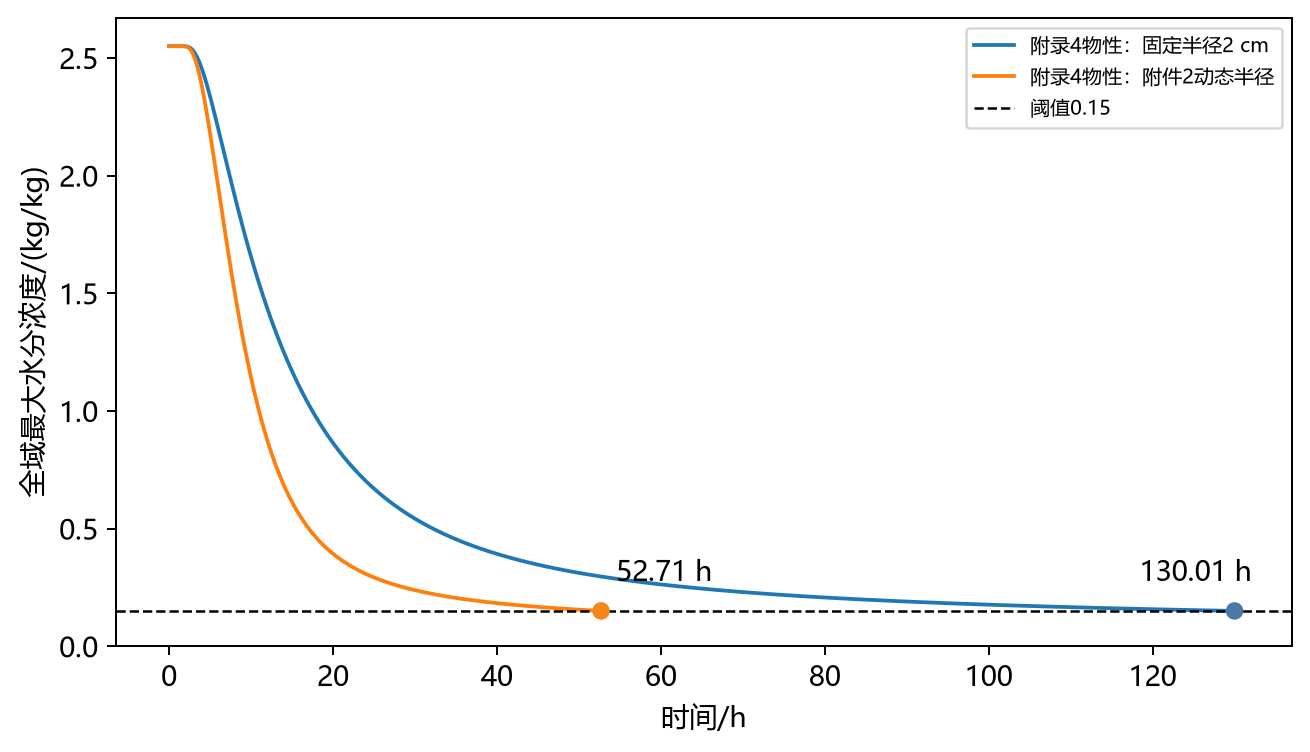
\includegraphics[width=0.82\textwidth]{shrinkage_effect.png}
\caption{附录4物性下固定半径（130.02 h）与动态收缩（52.72 h）的干燥历程对比}\label{fig:shrinkage}
\end{figure}
\begin{figure}[H]
\centering
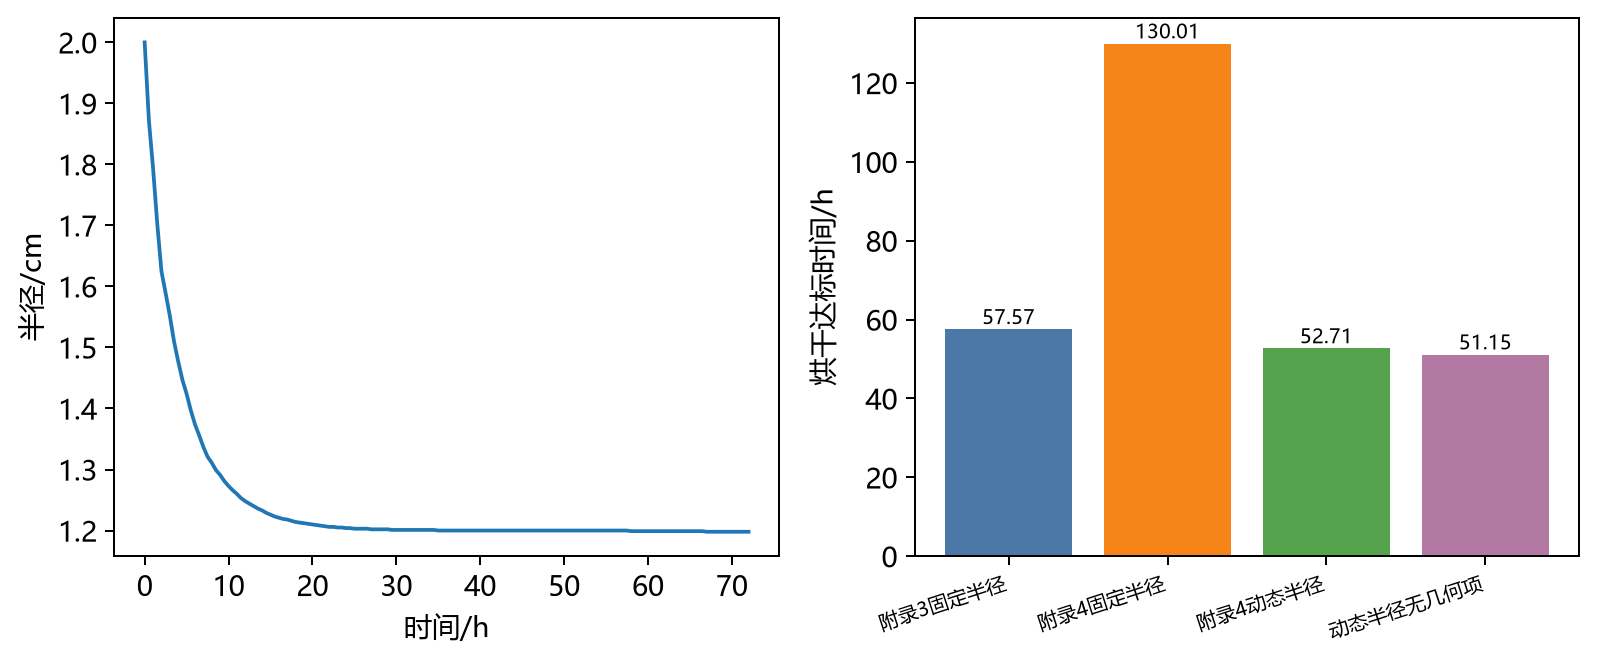
\includegraphics[width=0.92\textwidth]{radius_and_comparison.png}
\caption{附件2药材半径实测变化曲线（左）与不同模型烘干达标时间对比柱状图（右）}\label{fig:radius_comp}
\end{figure}

\subsubsection{坐标变换拟对流输运项的必要性与影响评估}
为评估将物理移动域映射至固定相对坐标时所产生的拟对流几何输运项 $\xi\frac{\dot{R}}{R}\frac{\partial\phi}{\partial\xi}$ 对计算精度的影响，设立敏感性对照算例：
\begin{itemize}
  \item \textbf{算例 D（输运项敏感性对照）}：采用附录4物性与附件2收缩，但在控制方程中人为略去该几何输运项（仅保留 $R^{-2}(t)$ 尺度缩放）。
\end{itemize}
计算表明，算例 D 的达标时长为 \NoCoordinateCaseHours\ h，相较完整模型（52.72 h）低估了 \OmitCoordinateDifference（约 2.98\%，绝对偏差达 1.57 h）。这定量证明：尽管该几何项不改变干燥总时长处于“约2.2天”的大数量级，但它对精确满足赛题四位小数精度要求具有决定性影响，在严谨的移动边界连续介质力学模拟中不可随意舍去。

\subsection{模型优缺点评价与改进展望}
\subsubsection{模型主要优点}
\begin{enumerate}[label=(\arabic*)]
  \item \textbf{框架高度统一且复用性强}：四问严格共享同一套基于广义守恒变量的空间半离散线方法体系，仅需切换对应的物性函数与边界条件，算法架构整洁优美；
  \item \textbf{严格保持局部与全局守恒性}：空间离散采用几何柱面加权的顶点中心有限体积法，内部界面通量形成严格的望远镜级数对消，机器浮点精度级别满足质量与能量守恒；
  \item \textbf{超刚性方程的高效极速求解}：引入两场三点紧凑模式的稀疏雅可比矩阵优化（CSR），配合自适应高阶 BDF 隐式积分推进，在保证绝对数值稳定性的前提下，实现长达 72 h 跨度物理全过程的秒级极速求解；
  \item \textbf{移动边界处理兼备严格性与实用性}：通过 Landau 相对坐标归一化彻底规避了动网格重划分的插值误差，完整保留了几何收缩双重机制，并构建了连续事件与 60 s 输出网格双重达标判定体系。
\end{enumerate}

\subsubsection{局限性与工业优化改进方向}
\begin{enumerate}[label=(\arabic*)]
  \item \textbf{相变潜热与热湿焓耦合效应未显式刻画}：模型将水分相变蒸发潜热并入了等效比热容与传热经验参数中，未来可进一步建立包含气--液--固三相平衡的非平衡态升华与汽化能量方程；
  \item \textbf{几何收缩本构关系有待内生化}：当前问题4基于实测几何数据驱动 $R(t)$。若能获得材料力学实验数据，可建立应力--应变与含水率直接关联的收缩本构方程 $R(C)$，实现热--质--固力学全耦合求解；
  \item \textbf{二维轴对称与端部效应深化}：对于长径比较小的短柱药材，两端面的吸热与排湿不可忽视，可进一步拓展至 $(r,z)$ 二维有限体积求解器。
\end{enumerate}

\subsection{结论与支撑材料复现说明}
\subsubsection{主要研究结论}
\begin{enumerate}[label=(\arabic*)]
  \item 烘干初期温度场在 30 min 内迅速建立并在 3 h 内高度接近热平衡，而水分场的迁移具有显著的时间滞后性，全过程由中心最晚达到阈值；
  \item 问题3固定半径下的全域烘干达标时刻为 \QThreeDryHours\ h（约 2.40 d）；问题4在附录4物性与动态收缩下的达标时刻为 \QFourDryHours\ h（约 2.20 d），终点尺寸为 \QFourDryRadius\ cm；
  \item 几何收缩是克服材料内部大扩散阻力的最关键驱动机制，能使干燥整体提速达 2.47 倍。
\end{enumerate}

\subsubsection{支撑材料组织与一键复现指南}
本研究交付的支撑材料采用模块化、轻量级与全流程一键复现架构，代码结构与文件组织如下：
\begin{enumerate}[label=(\arabic*)]
  \item \textbf{一键复现主入口（\texttt{run\_all.py}）}：依次自动调用核心求解器驱动四问计算、输出标准 Excel 工作簿（\texttt{result1.xlsx}--\texttt{result4.xlsx}）、执行敏感性分析并完成全套数据指标校验；
  \item \textbf{核心算法求解模块（\texttt{src/drying\_solver.py}）}：基于有限体积线方法与 SciPy 刚性 BDF 求解器实现全过程数值积分、稀疏雅可比模式构建、事件检测与图件渲染；
  \item \textbf{参数敏感性分析模块（\texttt{src/sensitivity\_analysis.py}）}：独立开展 $\pm 10\%$ 参数摄动实验并输出结构化指标；
  \item \textbf{依赖环境与运行}：依赖包仅需 NumPy、SciPy、openpyxl、Pandas 与 Matplotlib。在支撑材料目录下仅需运行命令：
  \begin{verbatim}
  python run_all.py
  \end{verbatim}
  即可在 1--2 分钟内确定性、无损地全自动复现论文中的全部数值解、图表与 Excel 结果。
\end{enumerate}

\begin{thebibliography}{9}
\bibitem{crank} Crank J. \textit{The Mathematics of Diffusion}. 2nd ed. Oxford: Clarendon Press, 1975.
\bibitem{patankar} Patankar S V. \textit{Numerical Heat Transfer and Fluid Flow}. New York: Hemisphere, 1980.
\bibitem{hairer} Hairer E, Wanner G. \textit{Solving Ordinary Differential Equations II: Stiff and Differential-Algebraic Problems}. 2nd ed. Berlin: Springer, 1996.
\bibitem{incropera} Incropera F P, DeWitt D P, Bergman T L, Lavine A S. \textit{Fundamentals of Heat and Mass Transfer}. 6th ed. Hoboken: Wiley, 2007.
\bibitem{mujumdar} Mujumdar A S, ed. \textit{Handbook of Industrial Drying}. 4th ed. Boca Raton: CRC Press, 2014.
\end{thebibliography}

\end{document}
